%%%%%%%%%%%%%%%%%%%%%%%%%%%%%%%%%%%%%%%%%
% Jacobs Landscape Poster
% LaTeX Template
% Version 1.0 (29/03/13)
%
% Created by:
% Computational Physics and Biophysics Group, Jacobs University
% https://teamwork.jacobs-university.de:8443/confluence/display/CoPandBiG/LaTeX+Poster
% 
% Further modified by:
% Nathaniel Johnston (nathaniel@njohnston.ca)
%
% This template has been downloaded from:
% http://www.LaTeXTemplates.com
%
% License:
% CC BY-NC-SA 3.0 (http://creativecommons.org/licenses/by-nc-sa/3.0/)
%
%%%%%%%%%%%%%%%%%%%%%%%%%%%%%%%%%%%%%%%%%
%---------------------------------------------------------------------
%   CONFIGURACION GENERAL
%---------------------------------------------------------------------
\documentclass[final]{beamer}
\usepackage[scale=1.24]{beamerposter} % Use the beamerposter package for laying out the poster
\usetheme{confposter} % Use the confposter theme supplied with this template
\usepackage{exscale}
%Configurando secciones ['Cuadros de texto' pa los cuates] hay de dos tipos
%1) El puro texto (Sin un marco)
\setbeamercolor{block title}{fg=purple,bg=white} % Bloques (Sin cuadro) - Titulo
\setbeamercolor{block body}{fg=black,bg=white} % Bloques - cuerpo
%2) El texto con marco
\setbeamercolor{block alerted title}{fg=white,bg=dblue!70} % Cuadros - Titulo
\setbeamercolor{block alerted body}{fg=black,bg=dblue!10} % Cuadros - Cuerpo

%-----------------------------------------------------------
% MEDIDAS DEL POSTER
%----------------------------------------------------------
% To set effective sepwid, onecolwid and twocolwid values, first choose how many columns you want and how much separation you want between columns
% In this template, the separation width chosen is 0.024 of the paper width and a 4-column layout
% onecolwid should therefore be (1-(# of columns+1)*sepwid)/# of columns e.g. (1-(4+1)*0.024)/4 = 0.22
% Set twocolwid to be (2*onecolwid)+sepwid = 0.464
% Set threecolwid to be (3*onecolwid)+2*sepwid = 0.708

\newlength{\sepwid}
\newlength{\onecolwid}
\newlength{\twocolwid}
\newlength{\threecolwid}
\setlength{\paperwidth}{48in} % Width 150 cm  [Max 96in - 244 cm]
\setlength{\paperheight}{36in} % Heighth 120.22 [Max 48 - 121 m]
\setlength{\sepwid}{0.01\paperwidth} % Separation width (white space) between columns
\setlength{\onecolwid}{0.24\paperwidth} % Width of one column
\setlength{\twocolwid}{0.464\paperwidth} % Width of two columns
\setlength{\threecolwid}{0.708\paperwidth} % Width of three columns
\setlength{\topmargin}{0in} % Reduce the top margin size
%-----------------------------------------------------------
% PAQUETES PA' HACER EL POSTER
%-------------------------------------------

\usepackage{graphicx}  % Required for including images
\usepackage[utf8]{inputenc}
\usepackage[portuges, brazil]{babel}   
\usepackage{booktabs} % Top and bottom rules for tables

%----------------------------------------------------------------------------------------
%   TITULO & LOGOS
%----------------------------------------------------------------------------------------

\title{Bayesian cognitive and statistical modeling applied to Signal Detection Theory and the Mirror Effect in a perceptual task.} % Poster title
\author{Adriana F. Chávez De la Peña; Michael D. Lee; Arturo Bouzas Riaño} % Author(s)
\institute{National Autonomous University of Mexico (UNAM); Faculty of Psychology\\ University of California Irvine} % Institution(s)

\begin{document}
\addtobeamertemplate{block end}{}{\vspace*{1.5ex}} % White space under blocks
\addtobeamertemplate{block alerted end}{}{\vspace*{1.5ex}} % White space under highlighted (alert) blocks
\setlength{\belowcaptionskip}{1ex} % White space under figures
\setlength\belowdisplayshortskip{1ex} % White space under equations
\begin{frame}[t] % The whole poster is enclosed in one beamer frame
\begin{tikzpicture}[remember picture,overlay]
\node[anchor=north west] at ([shift={(1cm,-2.5cm)}]current page.north west)
    {
\includegraphics[width=8.5cm]{Figures/UNAMiwi.png}};
\node[anchor=north east] at ([shift={(-1cm,-2.5cm)}]current page.north east)
    {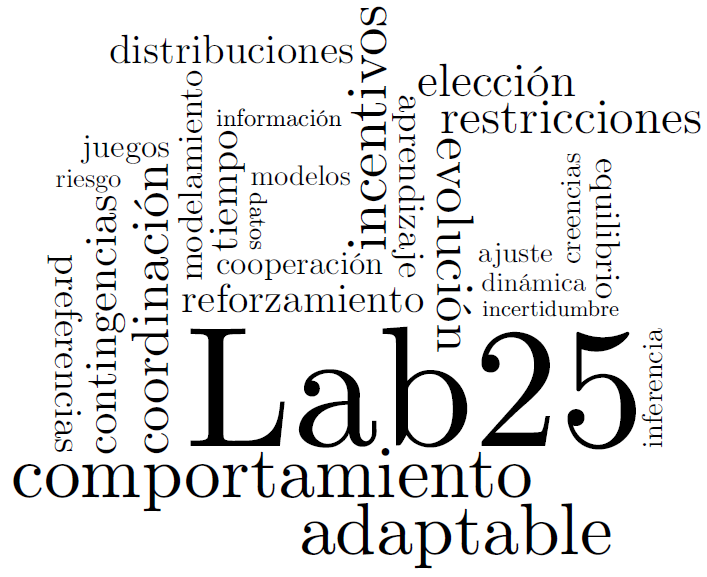
\includegraphics[height=11cm]{Figures/Lab25.png}};
\end{tikzpicture}

%----------------------------------------------------------------------------------------
%----------------------------------------------------------------------------------------
%   PRIMERA COLUMNA
%----------------------------------------------------------------------------------------
%   INTRODUCCION
%-------------------------------|||

\begin{columns}[t] % The whole poster consists of three major columns, the second of which is split into two columns twice - the [t] option aligns each column's content to the top
\begin{column}{\sepwid}\end{column} % Empty spacer column
\begin{column}{\onecolwid} % The first column

%jblue % jblue!10
\setbeamercolor{block alerted title}{fg=white,bg=Plum}
\setbeamercolor{block alerted body}{fg=black,bg=Plum!10}
\begin{alertblock}{Introduction}

The Mirror Effect is a well-established empirical result in Recognition Memory: when  subjects' performance is compared between two classes of stimuli, one known to be easier to recognize (A class) than the other (B class), this difference is reflected in the identification of both target and lure stimuli (Glanzer et al., 1993). The  implied order of the underlying distributions under a SDT framework is what gives these patterns the name of the "Mirror Effect".

\begin{equation}
FA(A) < FA(B) < Hits(B) < Hits(A)
\label{eqn:Rates}
\end{equation}


\begin{figure}
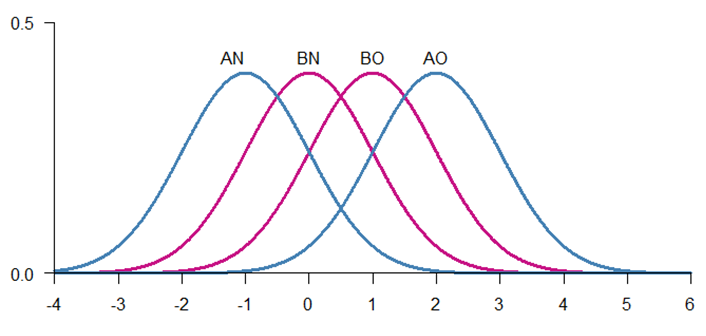
\includegraphics[width=0.4\linewidth]{Figures/MirrorEffect.png}
\end{figure}

\end{alertblock}


%------------------------------------------------------------------------------------------
% METODO & PROCEDIMIENTO
%-----------------------------------------|||||

\setbeamercolor{block alerted title}{fg=white,bg=Plum} % Titulo del Cuadro
\setbeamercolor{block alerted body}{fg=black,bg=Plum!10} % Cuerpo / Contenido del cuadro
\begin{alertblock}{Method: A perceptual task}
\textbf{To assess the generalizability of the Mirror Effect}, we designed a perceptual task where  the Ebbinghaus illusion, is used to construct the two classes of stimuli, A and B (Massaro \& Anderson  1971):
\begin{itemize}
\item A class ("Easier"): 2 or 3 surrounding circles - Weak illusion
\item B class ("Hard"): 7 or 8 surrounding circles - Strong illusion
\end{itemize}
$\quad$\\
\setbeamercolor{item}{fg=Purple}
\setbeamercolor{item projected}{fg=white,bg=Purple}
\begin{enumerate}
\item \textbf{Detection Task:} Are the central circles the same size?\\
\textbf{Two experiments:} 
\begin{itemize}
\item Experiment 1: Just one Ebbinghaus illusion on screen.
\item Experiment 2: Both circles were Ebbinghaus illusions.\\
\end{itemize}
\begin{center}
\begin{tabular}{ccc}
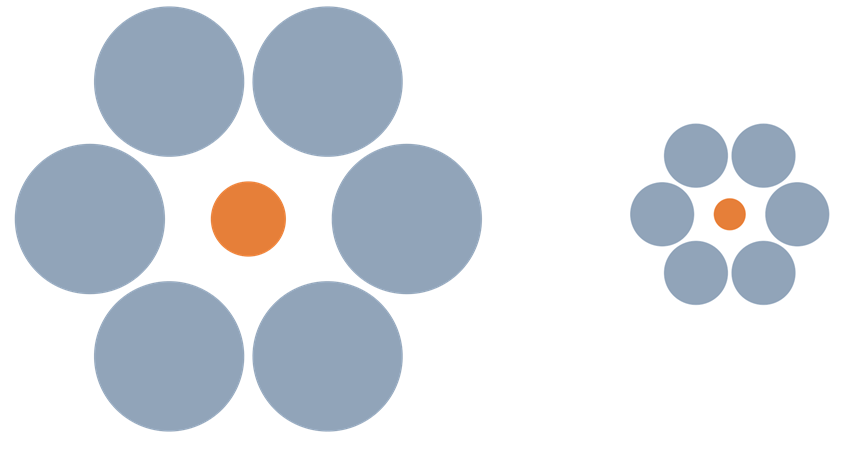
\includegraphics[width=0.35\linewidth]{Figures/MainTask3.png}
\end{tabular}
\end{center}
$\quad$\\
\item \textbf{Confidence Rating:} How certain are you of your previous response? (1-3 scale)
\end{enumerate}
\end{alertblock}


\setbeamercolor{block alerted title}{fg=white,bg=Plum}
\setbeamercolor{block alerted body}{fg=black,bg=Plum!10}
\begin{alertblock}{Replication of the original data analysis}
We found evidence for the Mirror Effect response rates in at least 85\% of our participants: In Experiment 1 we had 17/20 in the Yes/No task and 18/20 on their Confidence ratings; 19/20 participants did in Experiment 2, for both tasks). We conducted a step by step replication of the mean-based analysis reported in the literature (Glanzer $\&$ Adams, 1990), and found that:
\setbeamercolor{item}{fg=Purple}
\setbeamercolor{item projected}{fg=white,bg=Purple}
\begin{enumerate}
\item Differences among d' are statistically significant \\
($d'(A) > d'(B)$)
\item Differences among response rates are significant too ($H(A)>H(B) \& FA(A)<FA(B)$)
\item Differences among ratings are significant ($H(A)>H(B) \& FA(A)<FA(B)$)
\end{enumerate}
\end{alertblock} 


%-----------------------------------------------------------------------------------------
% FIN PRIMERA COLUMNA
%-----------------------------------------------------------------------------------------

\end{column} % End of the first column
\begin{column}{\sepwid}\end{column} % Empty spacer column
\begin{column}{\twocolwid} % Begin a column which is two columns wide (column 2)


%----------------------------------------------------------------------------------------
% RESULTADOS GENERALES
%----------------------------------------------------------------------------------------

\setbeamercolor{block alerted title}{fg=white,bg=MidnightBlue}
\setbeamercolor{block alerted body}{fg=black,bg=Plum!10}
\begin{alertblock}{A Bayesian approximation}
Given the probabilistic nature of the SDT model, it seems like the study of the Mirror Effect can benefit from the application of Bayesian statistical and cognitive modeling to evaluate the differences observed in the performance of participants across each class of stimuli.
\end{alertblock} 

%----------------------------------------------------------------------------------------
%   ANALISIS POR REPLICA 
%-------------------------------||||||||
\setlength{\onecolwid}{0.24\paperwidth}
\begin{columns}[t,totalwidth=\twocolwid] % Split up the two columns wide column
\begin{column}{\onecolwid}\vspace{-.6in} % The first column within column 2 (column 2.1)


\setbeamercolor{block alerted title}{fg=white,bg=MidnightBlue} % Change the alert block title colors
\setbeamercolor{block alerted body}{fg=black,bg=white} % Change the alert block body colors
\begin{alertblock}{}

\setbeamercolor{item}{fg=Purple}
\setbeamercolor{item projected}{fg=white,bg=Purple}
\begin{enumerate}
\item We apply a Hierarchical SDT model to see our data
\begin{center}
\begin{tabular}{ccc}
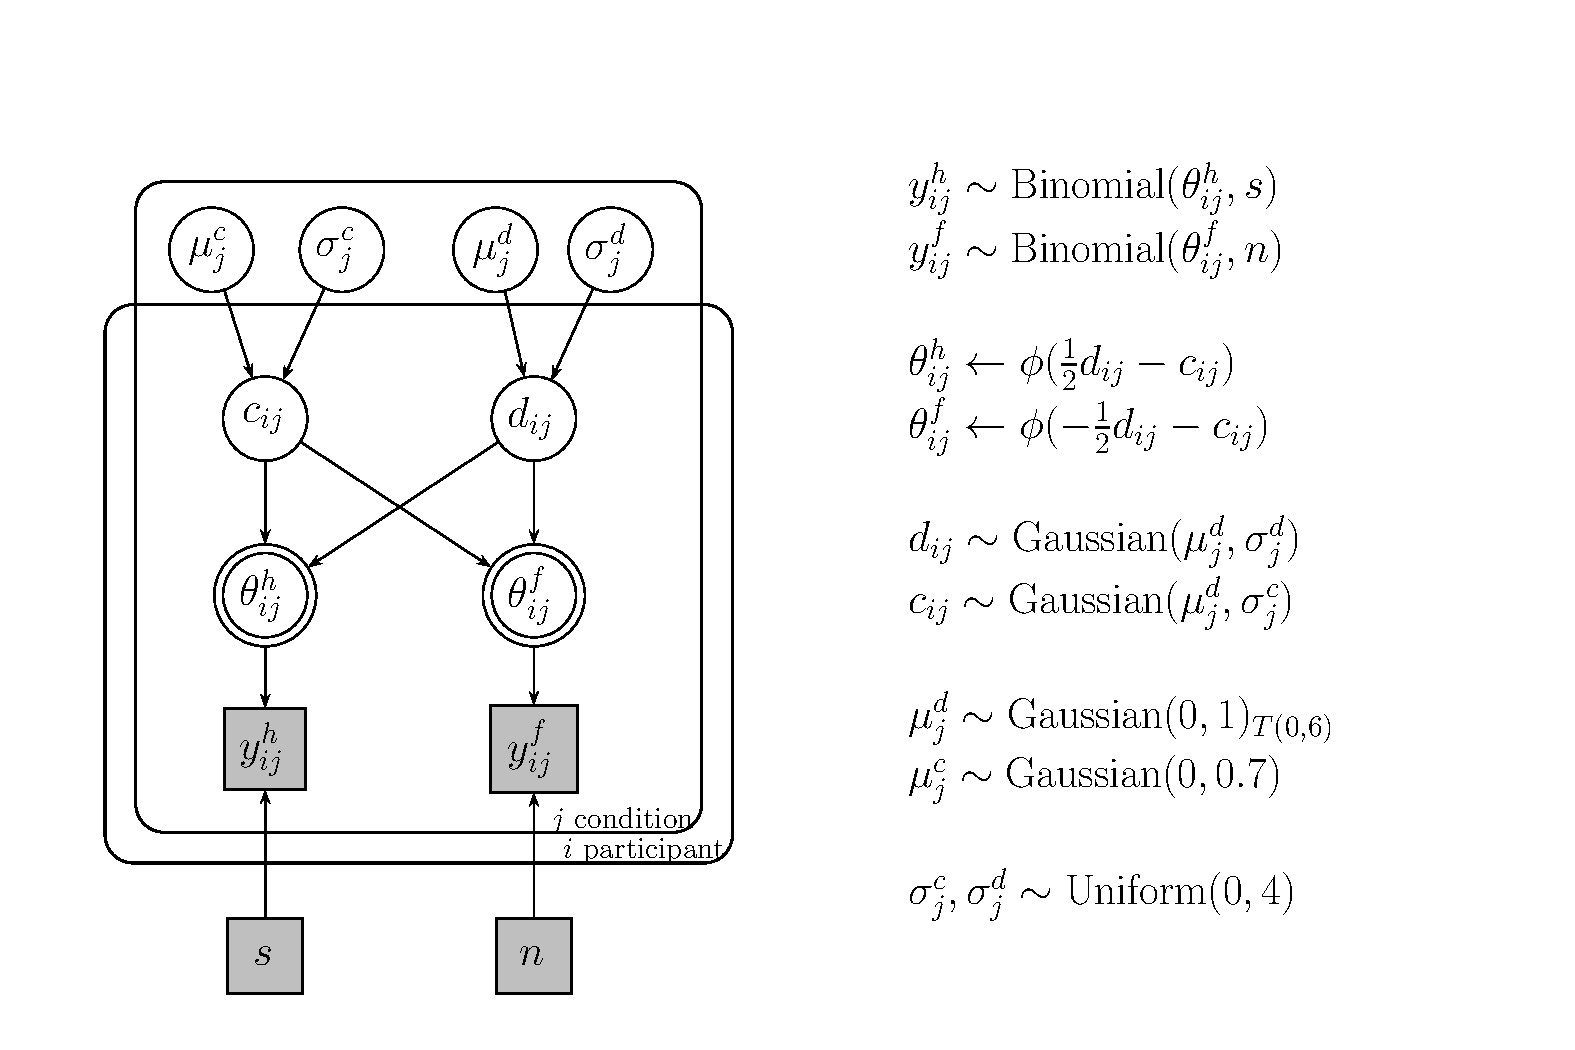
\includegraphics[width=0.65\linewidth]{Figures/0_HierarchicalSDT.pdf}
\end{tabular}
\end{center}

\begin{center}
\begin{tabular}{ccc}
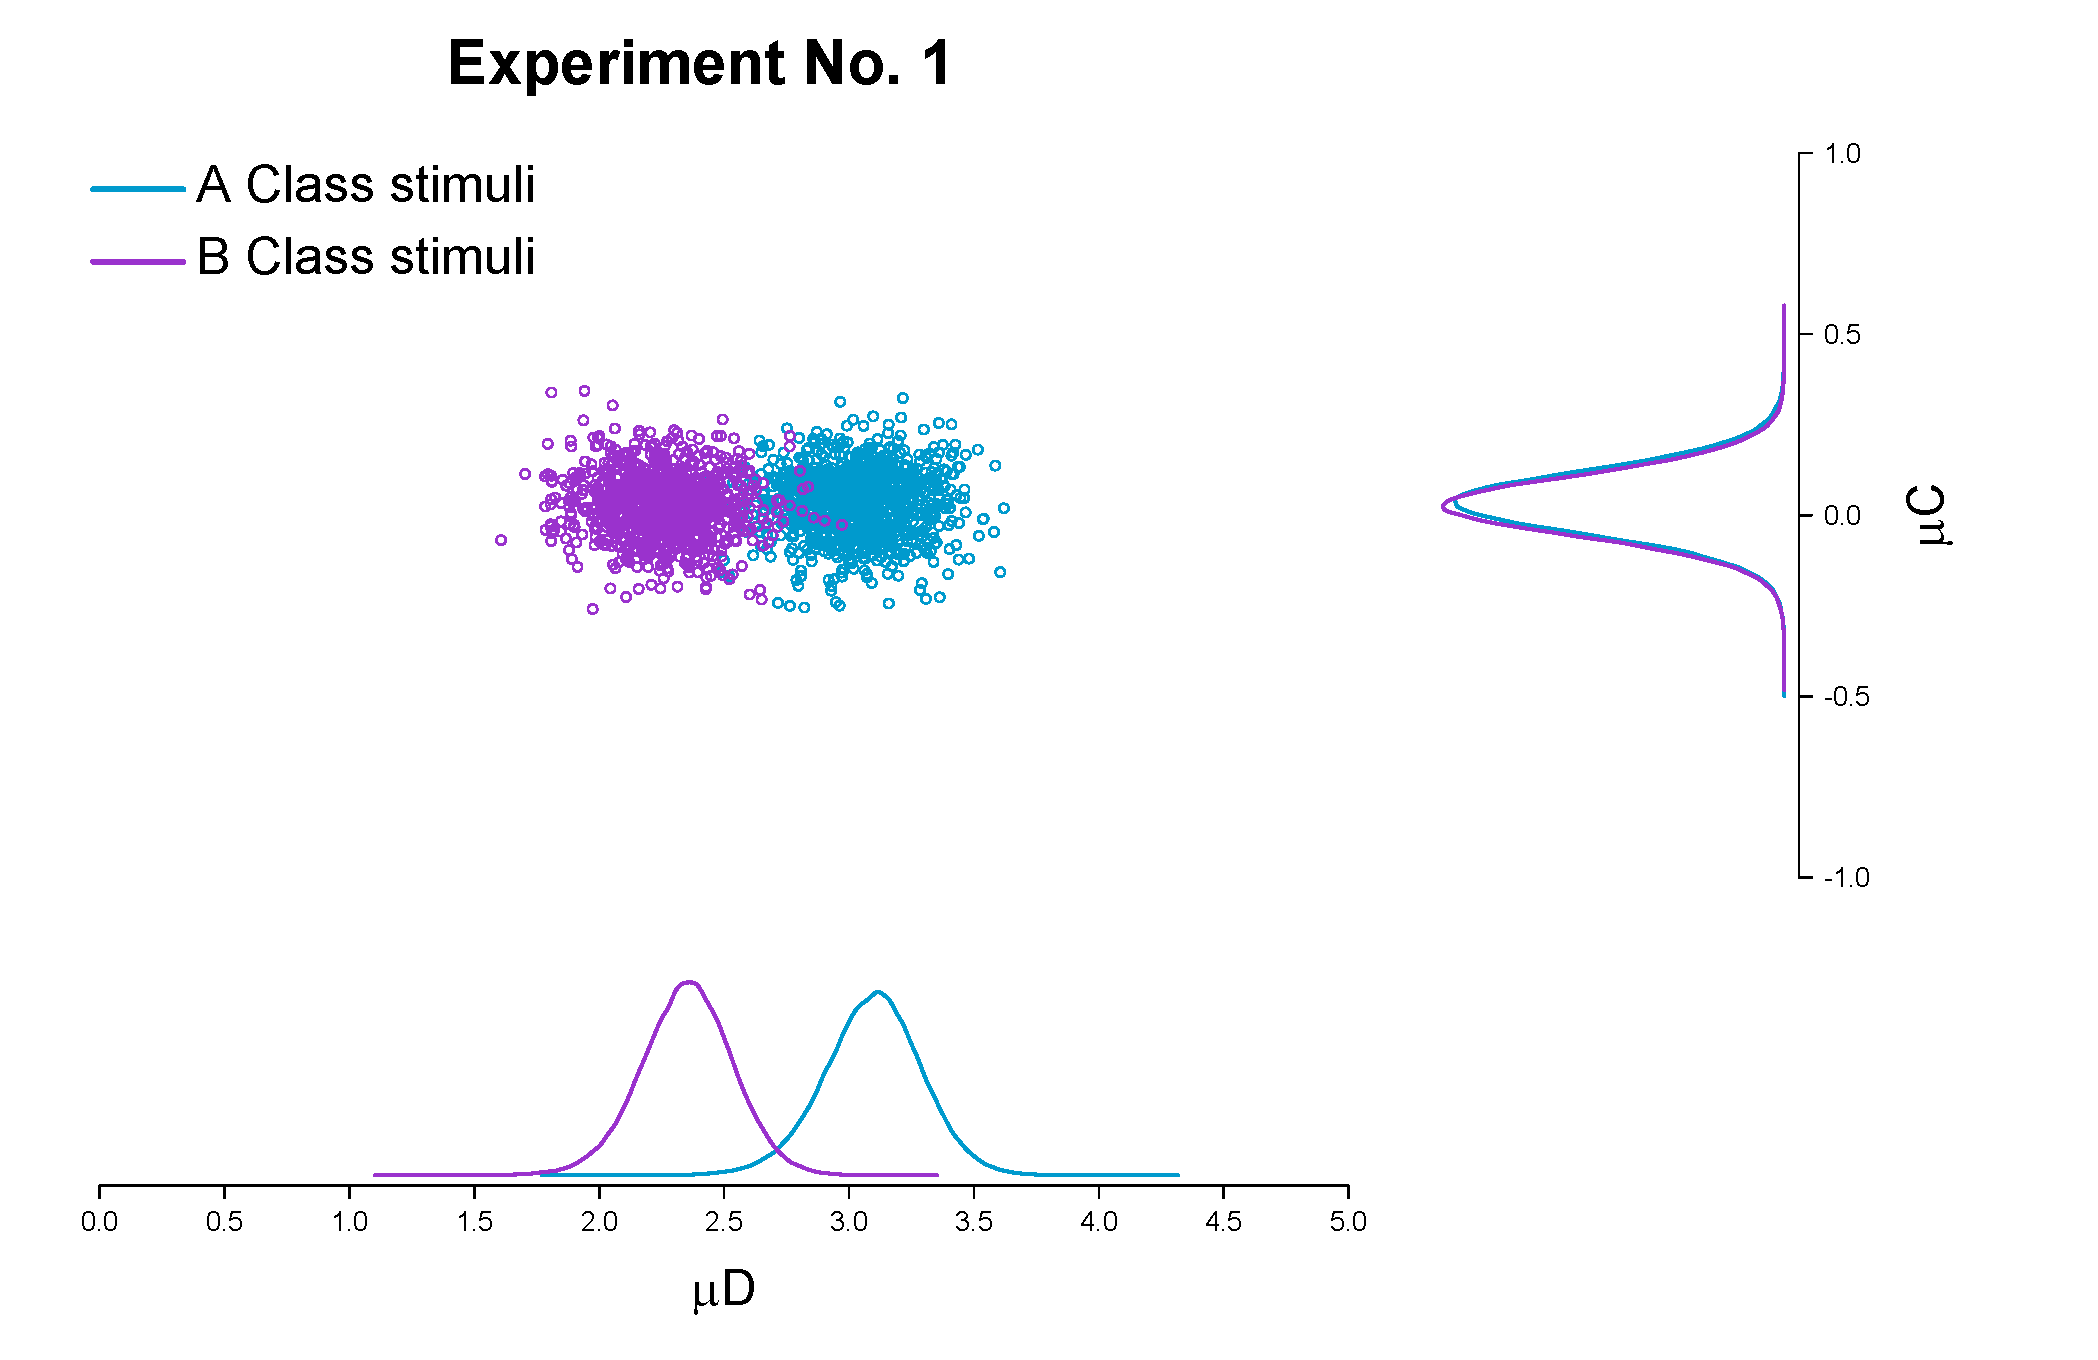
\includegraphics[width=0.47\linewidth]{Figures/0-Exp1.pdf} & \hfill & 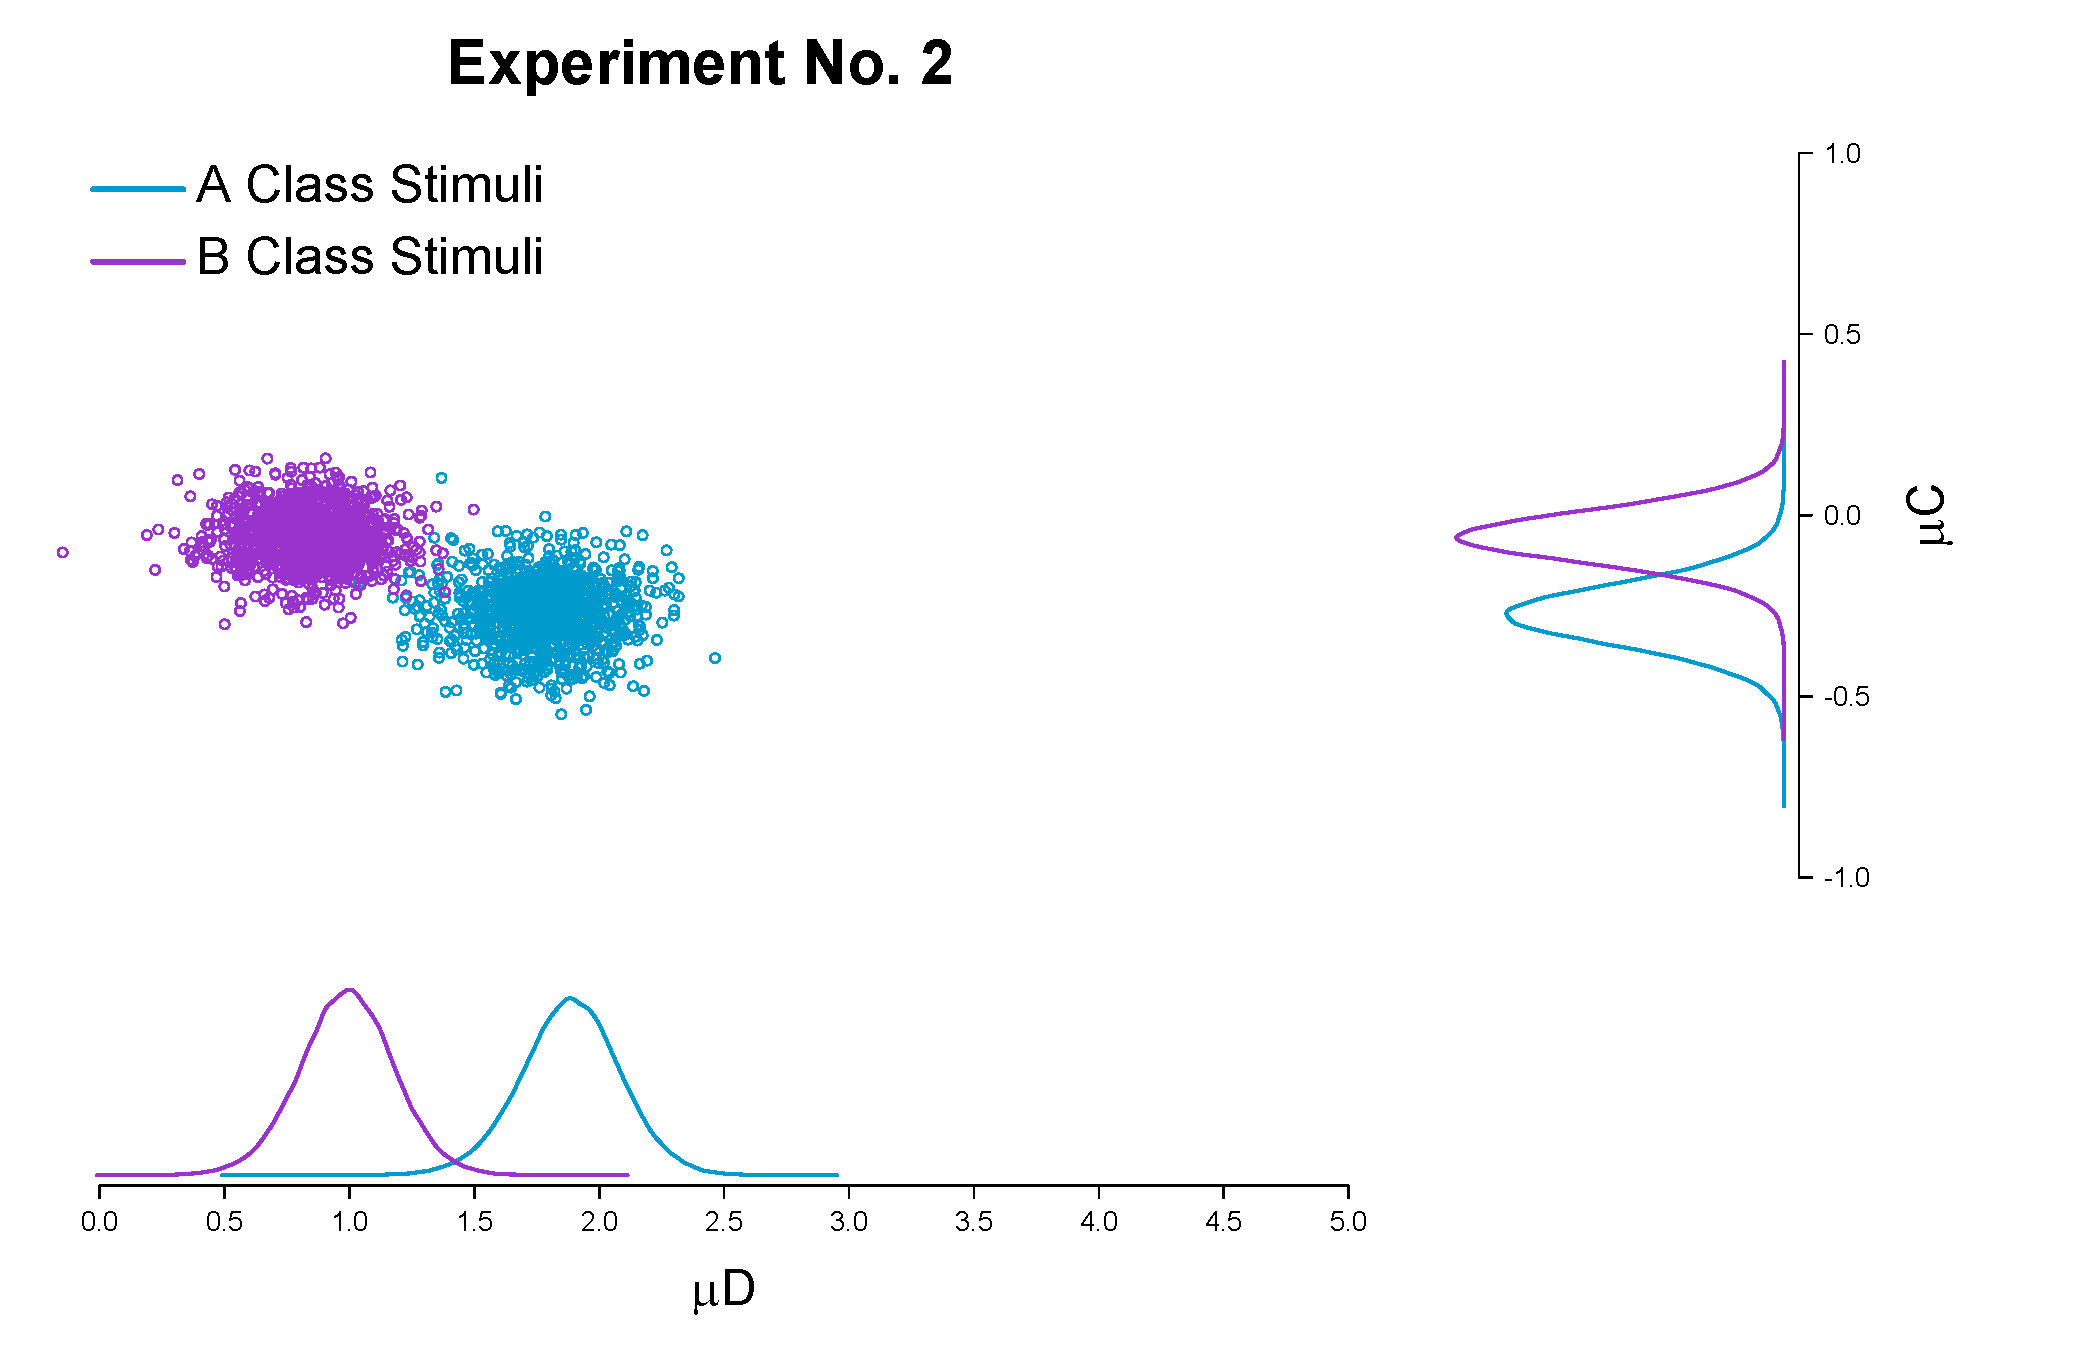
\includegraphics[width=0.47\linewidth]{Figures/0-Exp2.pdf}
\end{tabular}
\end{center}

$\qquad$

\item We test the differences across d'
\begin{center}
\begin{tabular}{ccc}
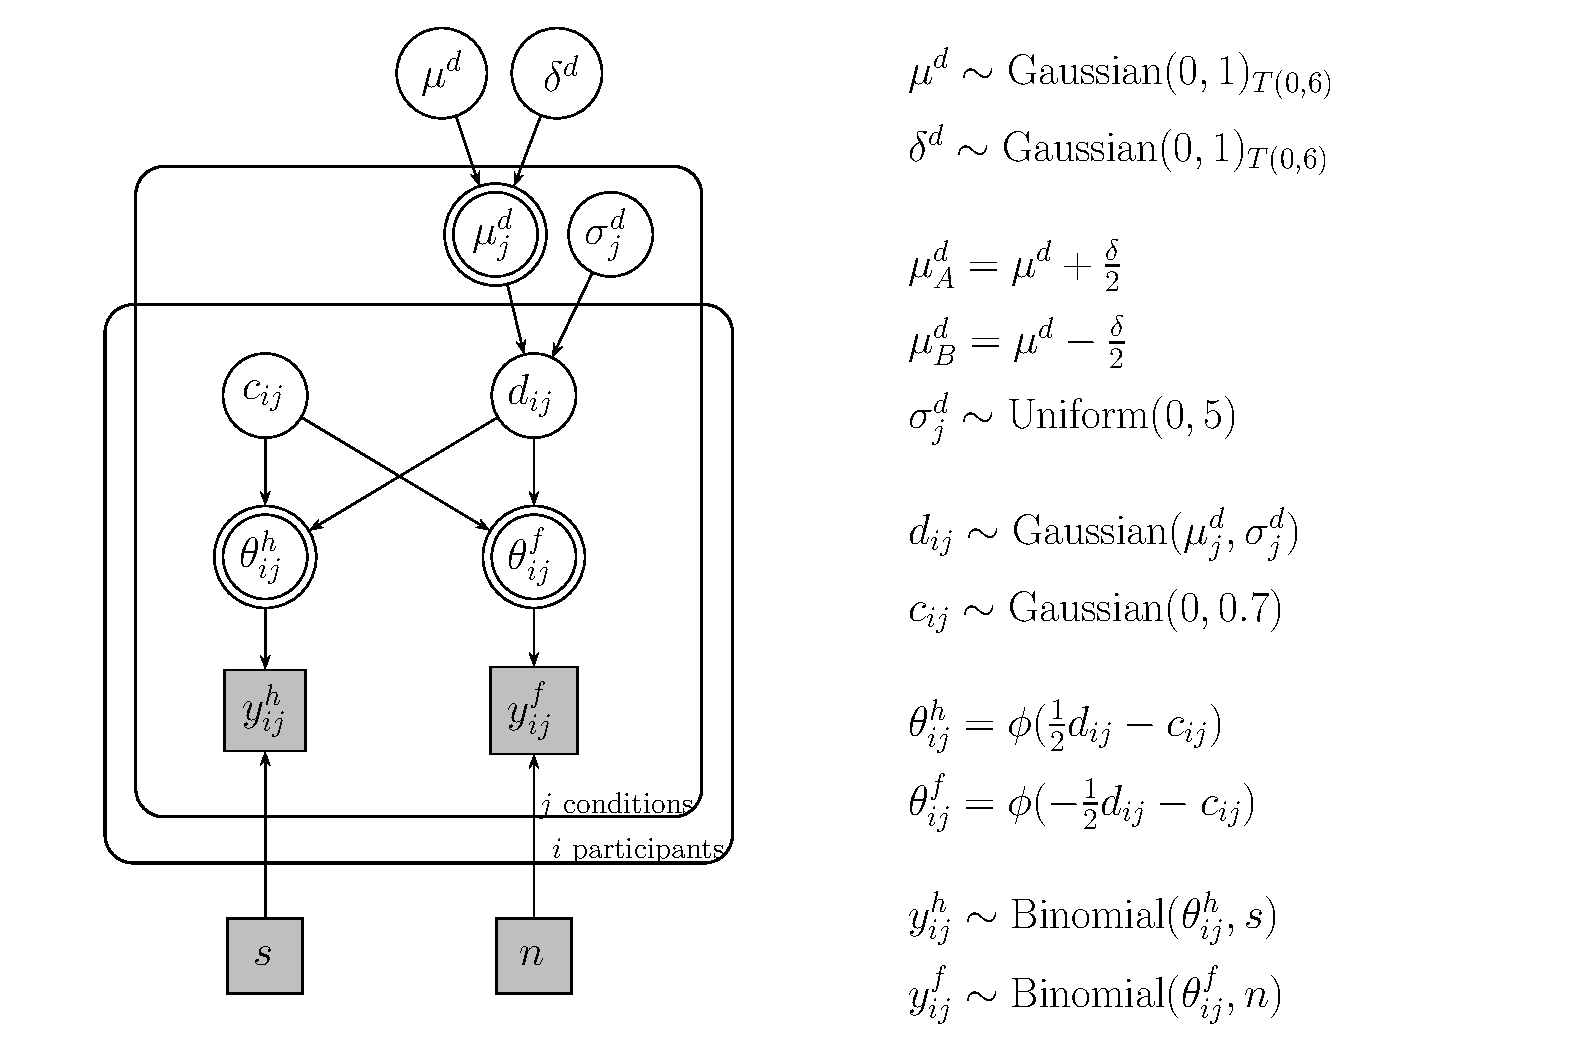
\includegraphics[width=0.7\linewidth]{Figures/1_DiffD.pdf}
\end{tabular}
\end{center}

\begin{center}
\begin{tabular}{ccc}
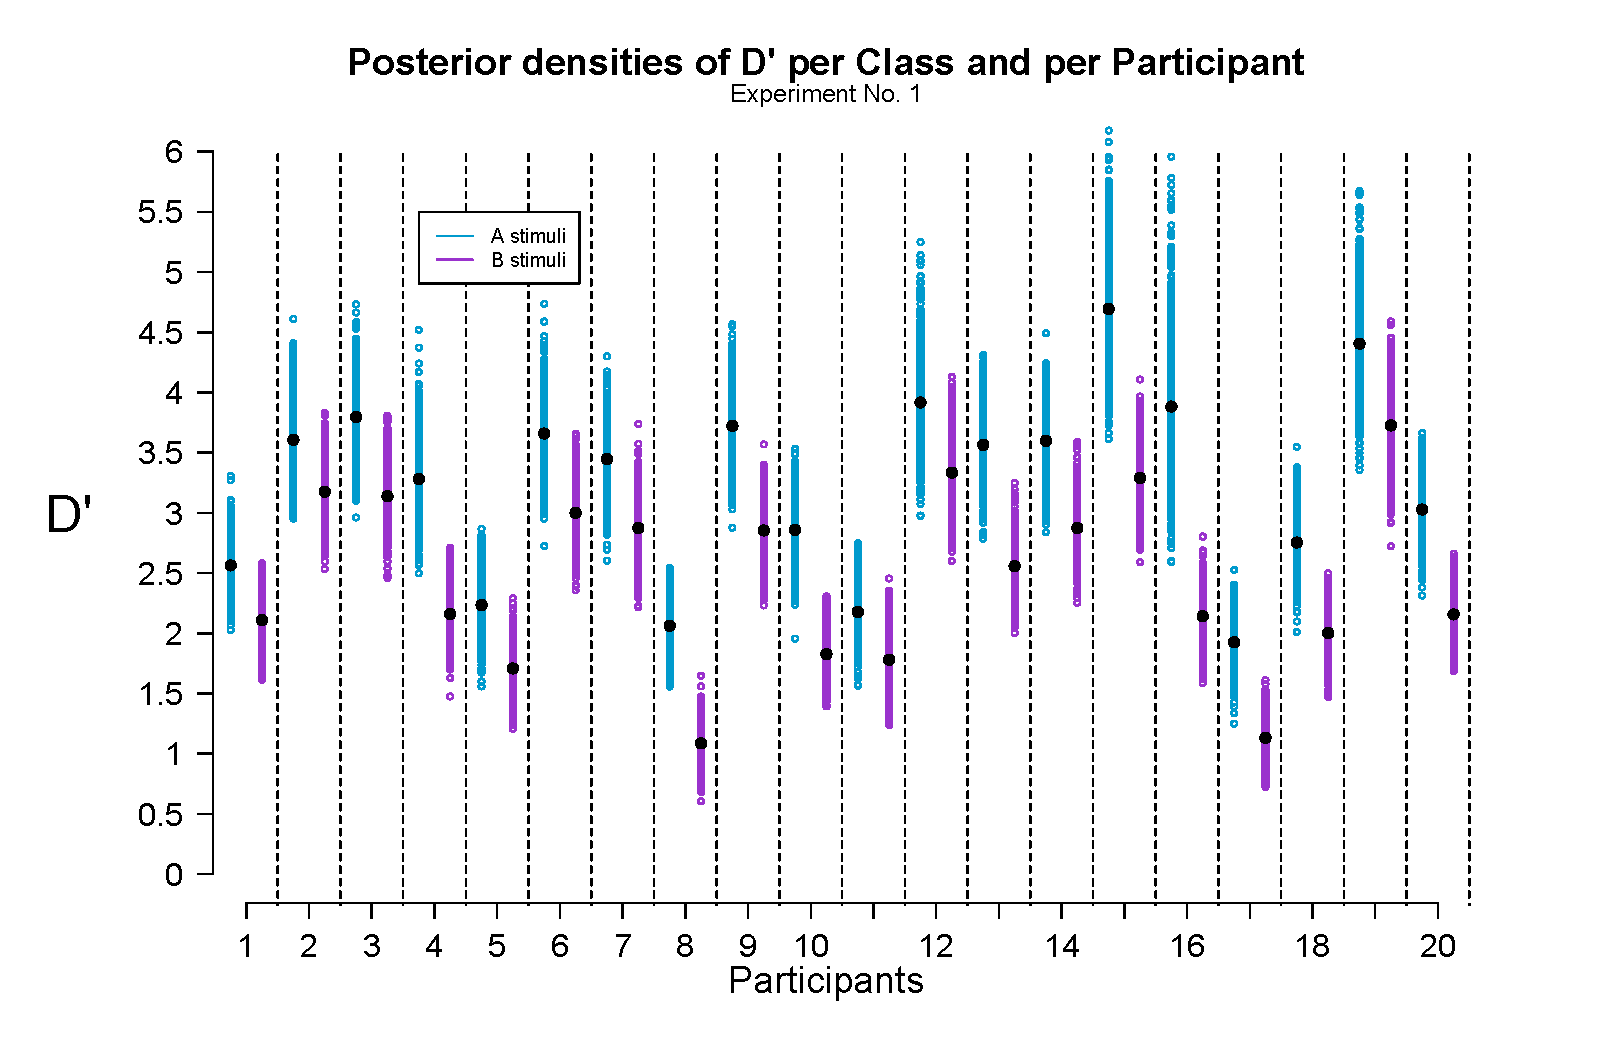
\includegraphics[width=0.5\linewidth]{Figures/1-Exp1_1.pdf} & \hfill & 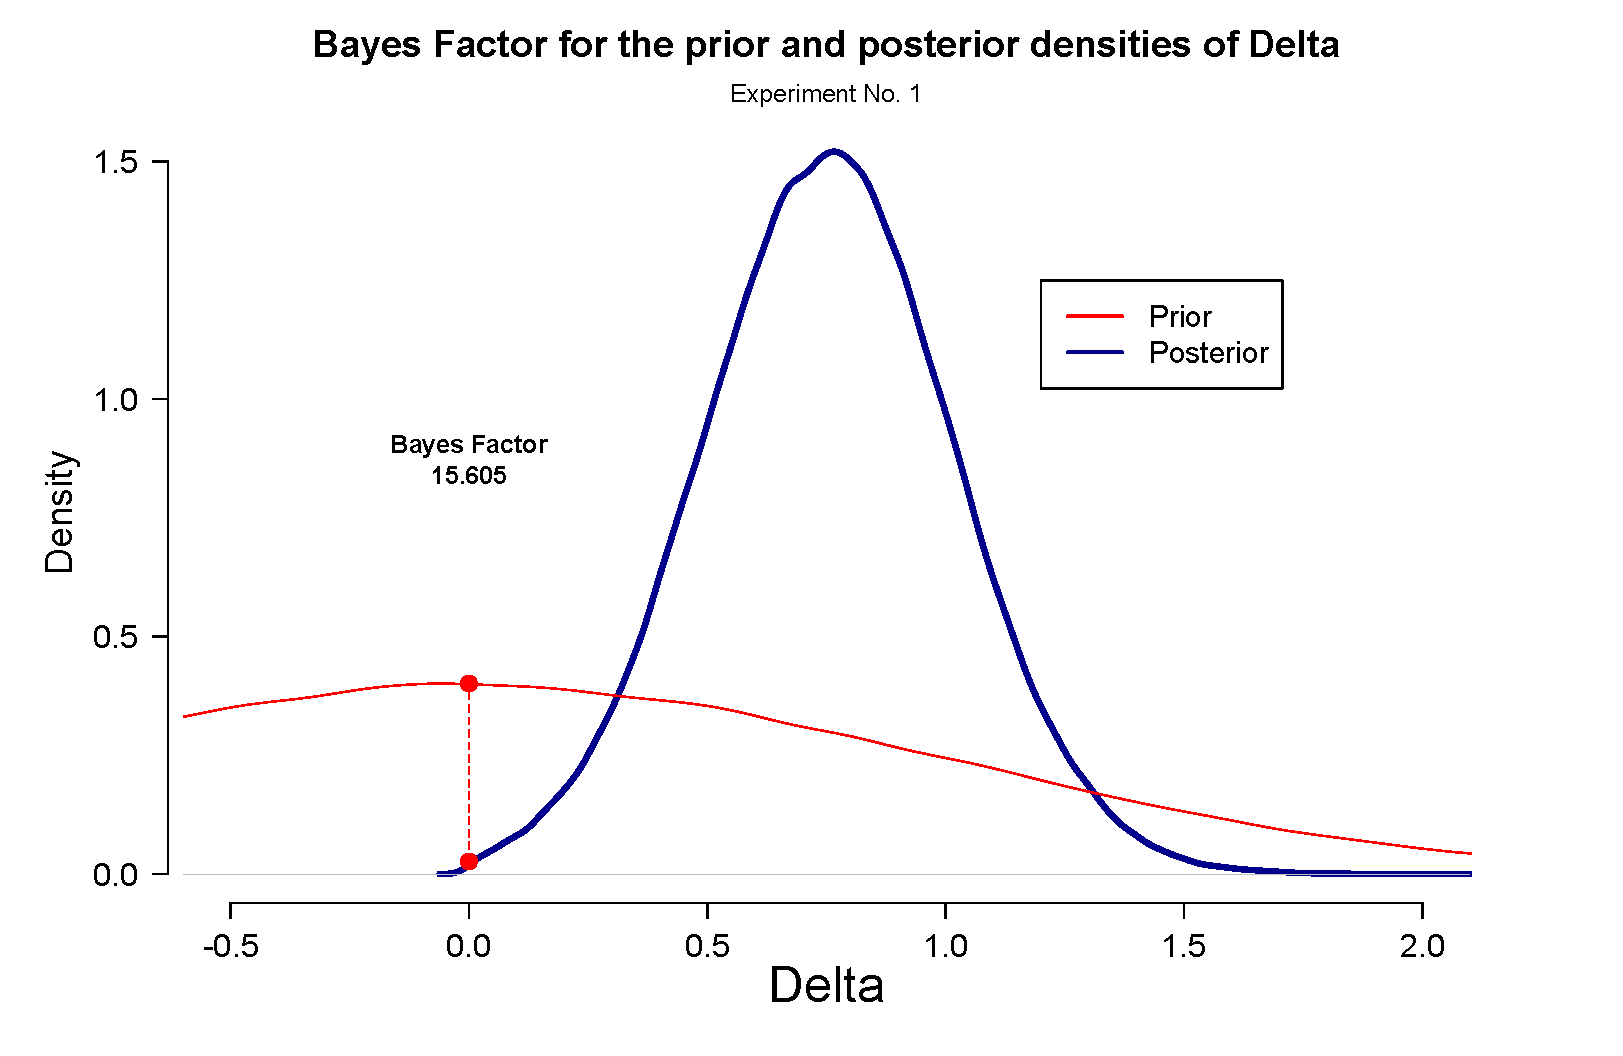
\includegraphics[width=0.45\linewidth]{Figures/1-Exp1_2.pdf}
\end{tabular}
\end{center}

\begin{center}
\begin{tabular}{ccc}
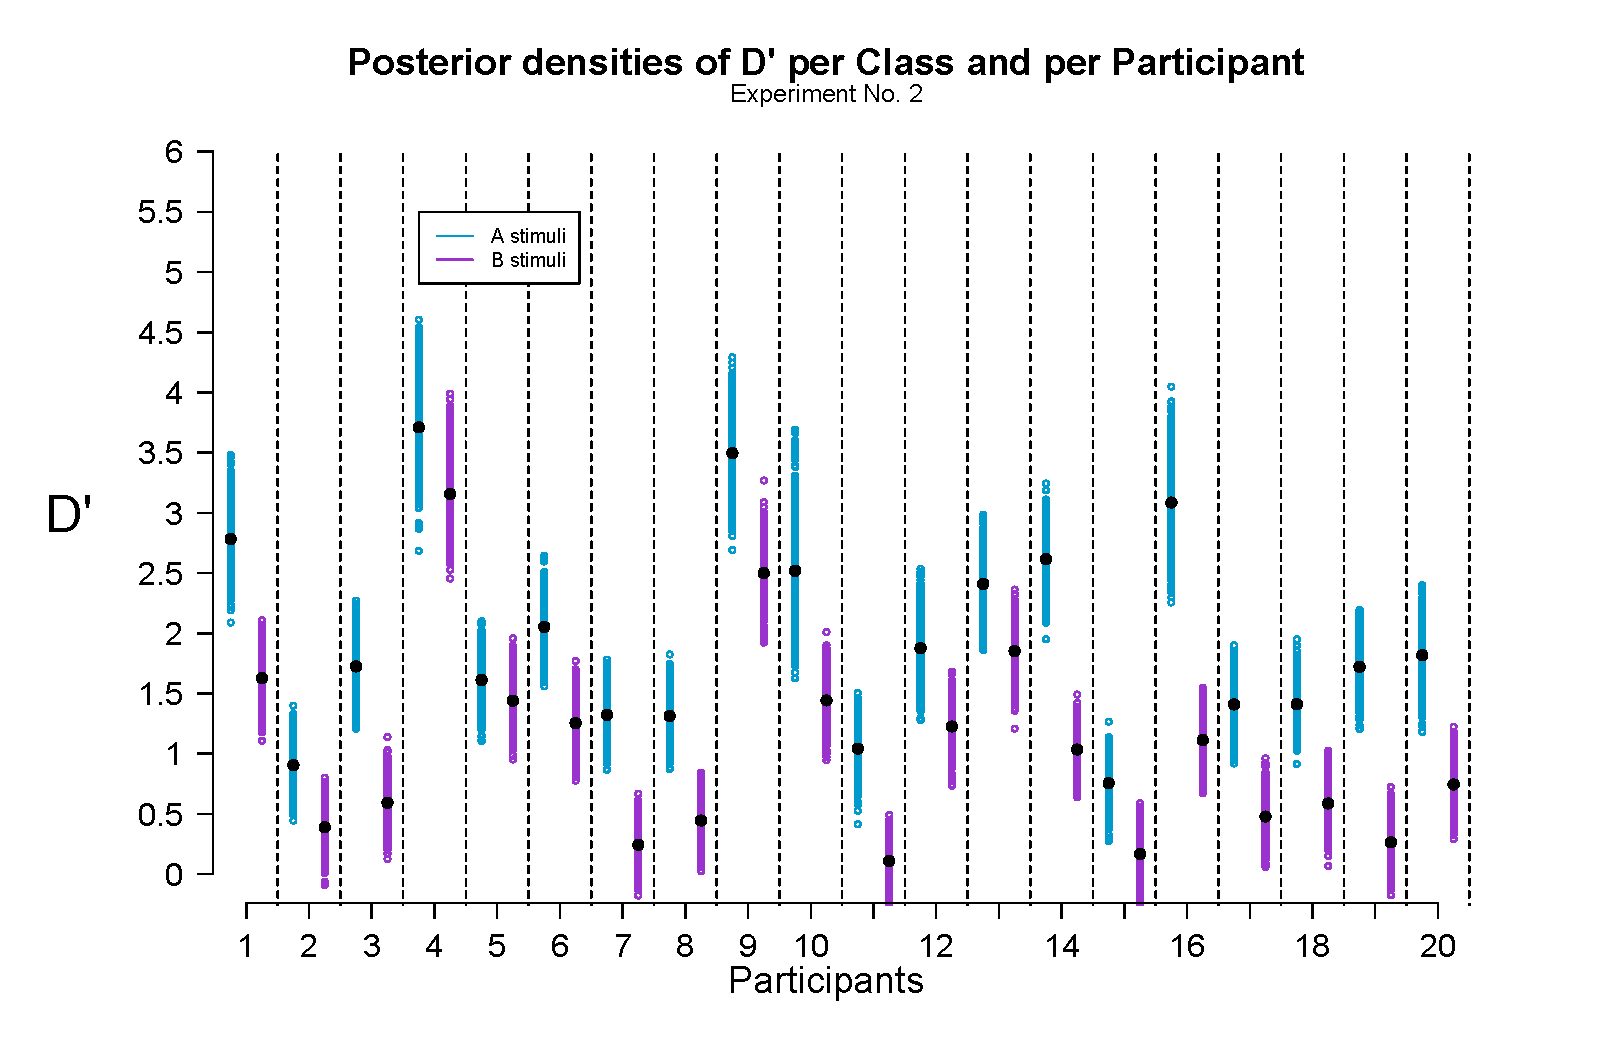
\includegraphics[width=0.5\linewidth]{Figures/1-Exp2_1.pdf} & \hfill & 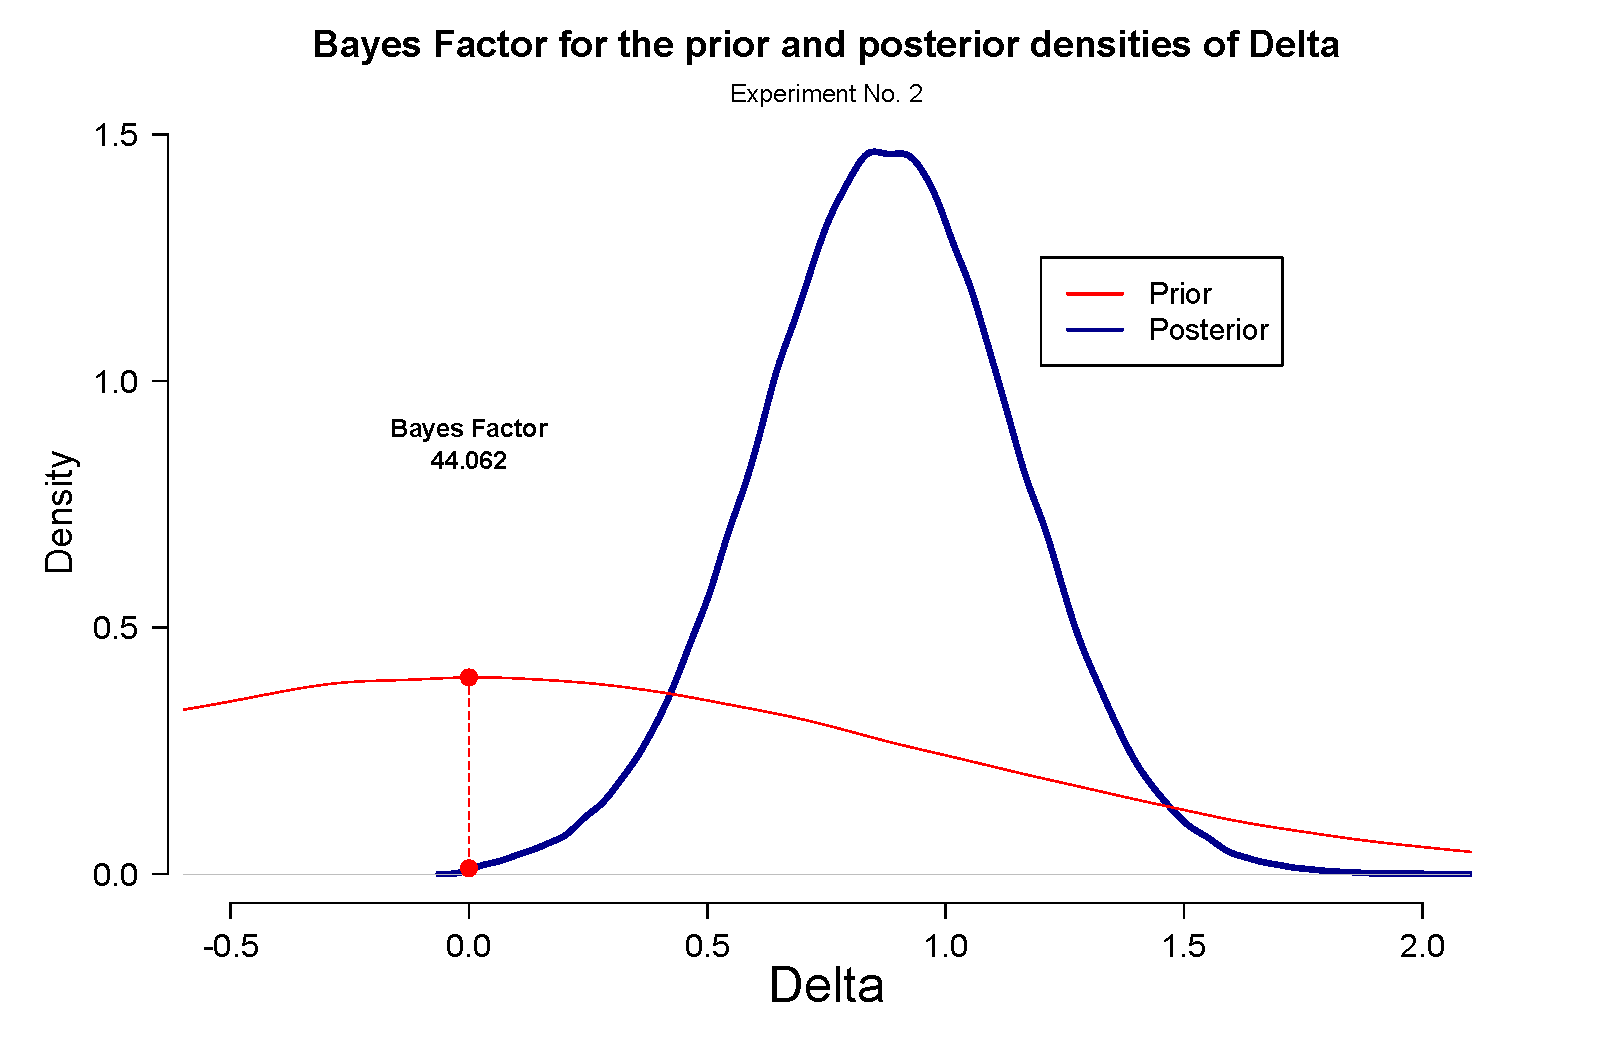
\includegraphics[width=0.45\linewidth]{Figures/1-Exp2_2.pdf}
\end{tabular}
\end{center}


\end{enumerate}
\end{alertblock}
\end{column} % End of column 2.1
%----------------------------------------------------------------------------------------

%----------------------------------------------------------------------------------------
%   BAYESIAN MODELING 
%----------------------------------------------------------------------------------------
\setlength{\onecolwid}{0.21\paperwidth}
\begin{column}{\sepwid}\end{column} % Empty spacer column
\begin{column}{\onecolwid}\vspace{-.6in} % The second column within column 2 (column 2.2)




\setbeamercolor{block alerted title}{fg=white,bg=MidnightBlue} % Change the alert block title colors
\setbeamercolor{block alerted body}{fg=black,bg=white} % Change the alert block body colors
\begin{alertblock}{}

\setbeamercolor{item}{fg=Purple}
\setbeamercolor{item projected}{fg=white,bg=Purple}
\begin{enumerate}
\item Are the Hit and F.A. rates different?
\end{enumerate}
\begin{center}
\begin{tabular}{ccc}
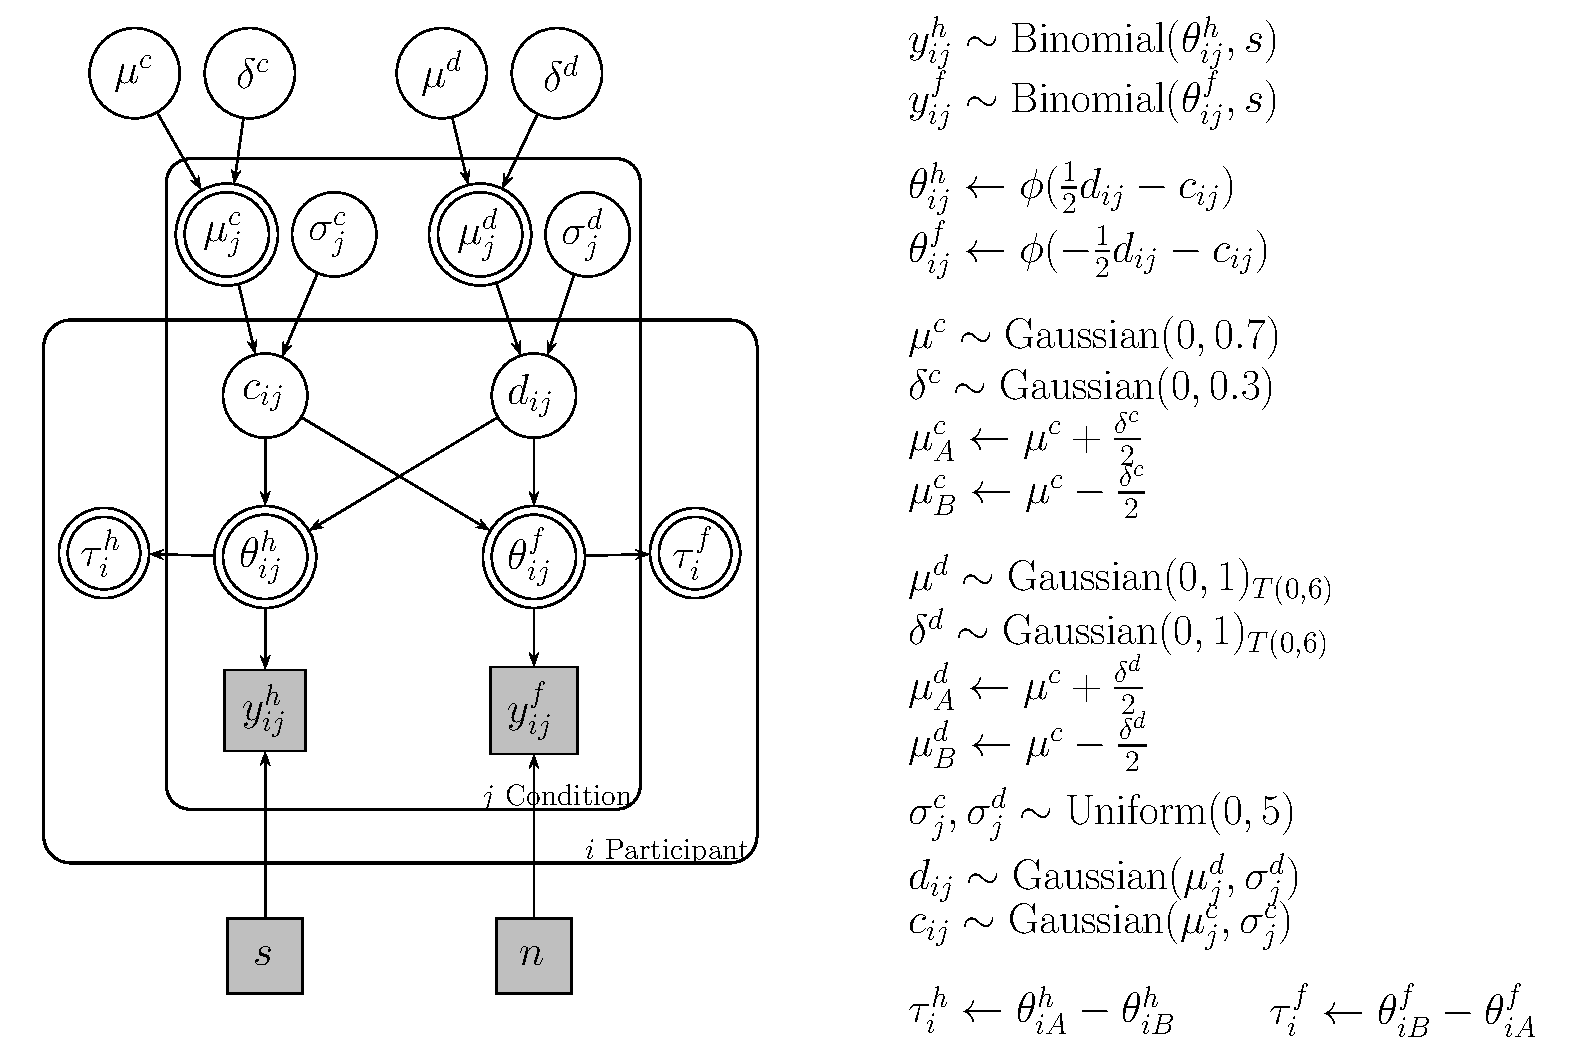
\includegraphics[width=0.9\linewidth]{Figures/3_Taus.pdf}
\end{tabular}
\end{center}

\begin{center}
\begin{tabular}{ccc}
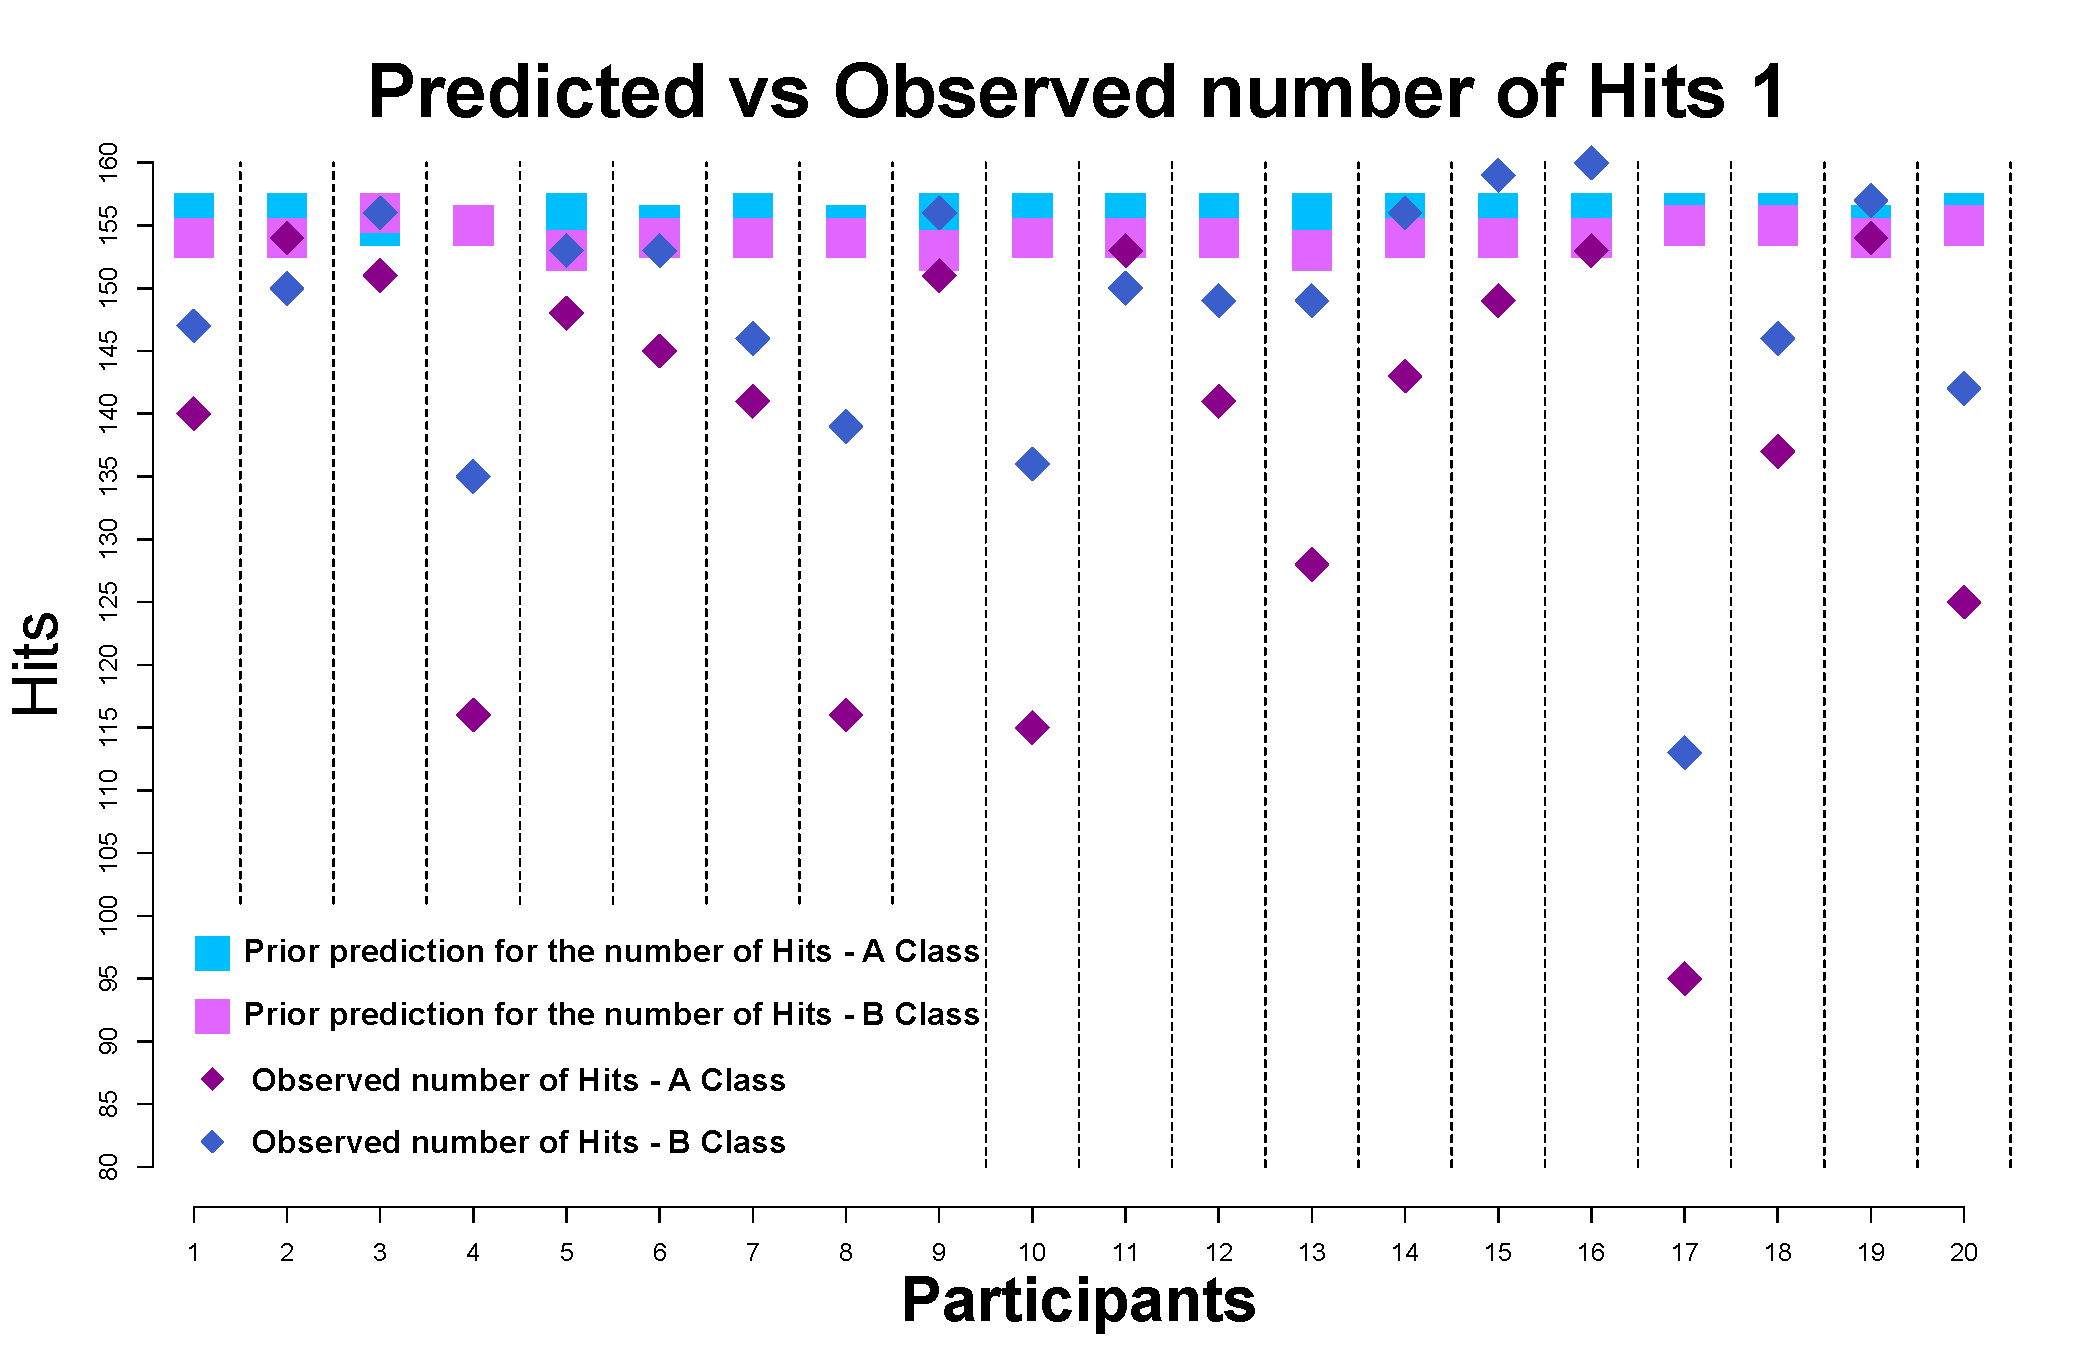
\includegraphics[width=0.45\linewidth]{Figures/3-PredictionsH.pdf} & \hfill & 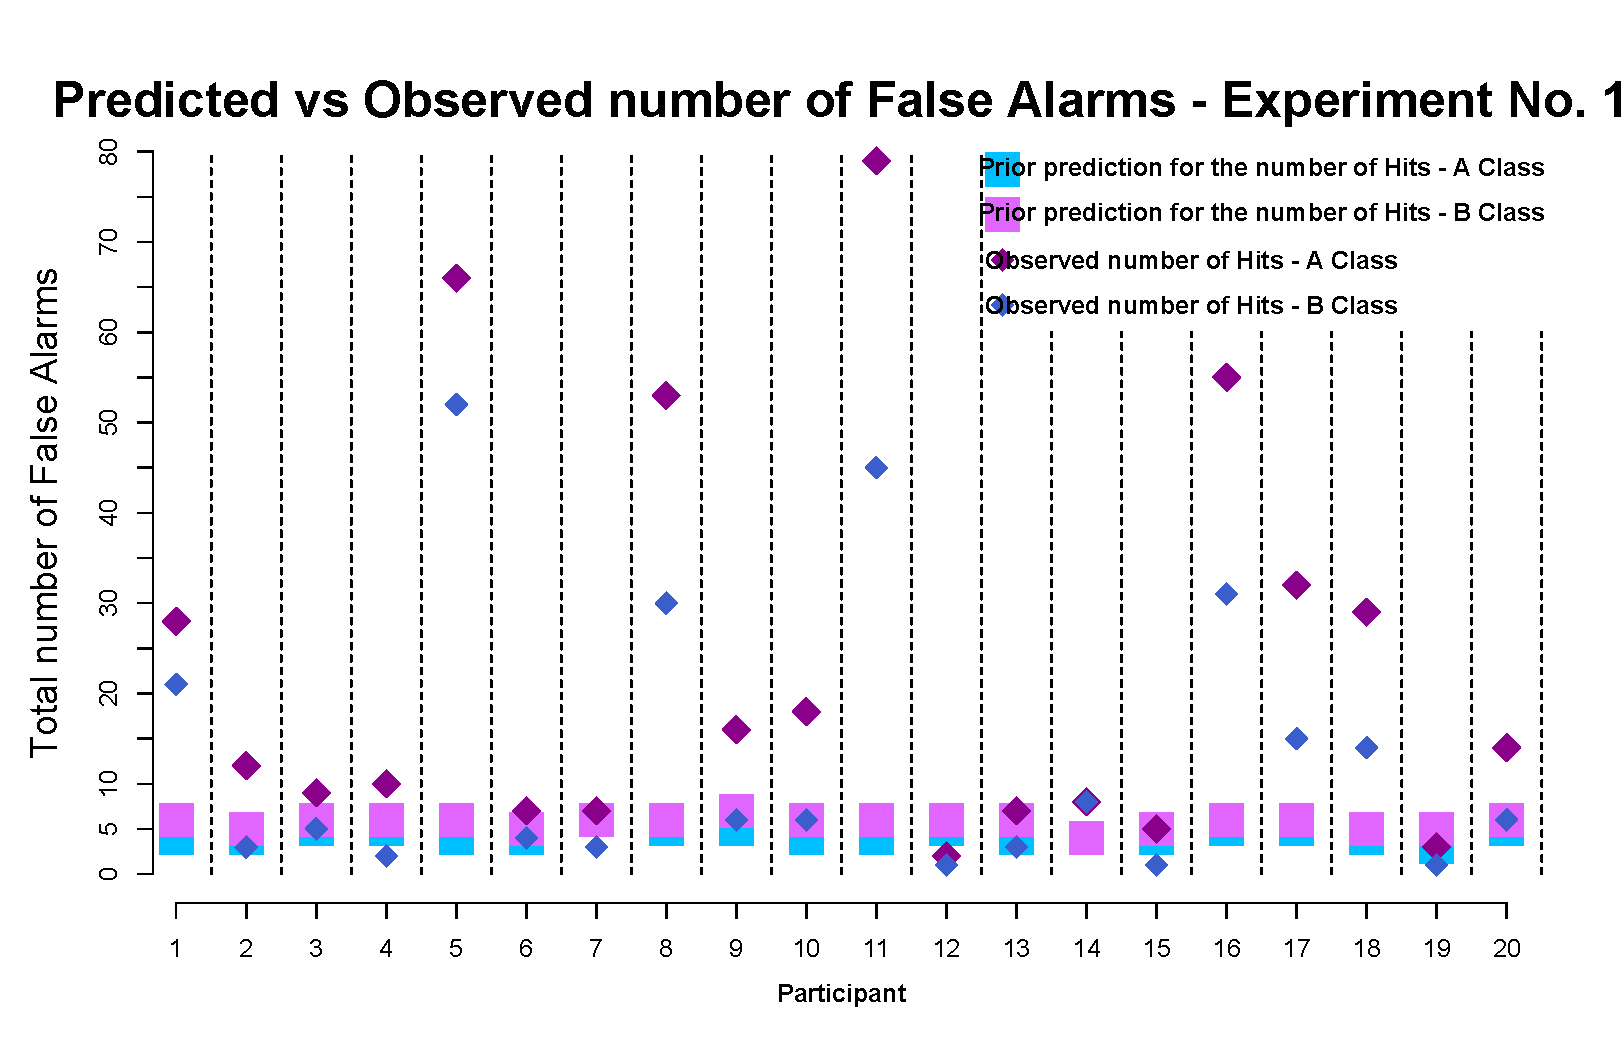
\includegraphics[width=0.45\linewidth]{Figures/3-PredictionsF.pdf}
\end{tabular}
\end{center}

\begin{center}
\begin{tabular}{ccc}
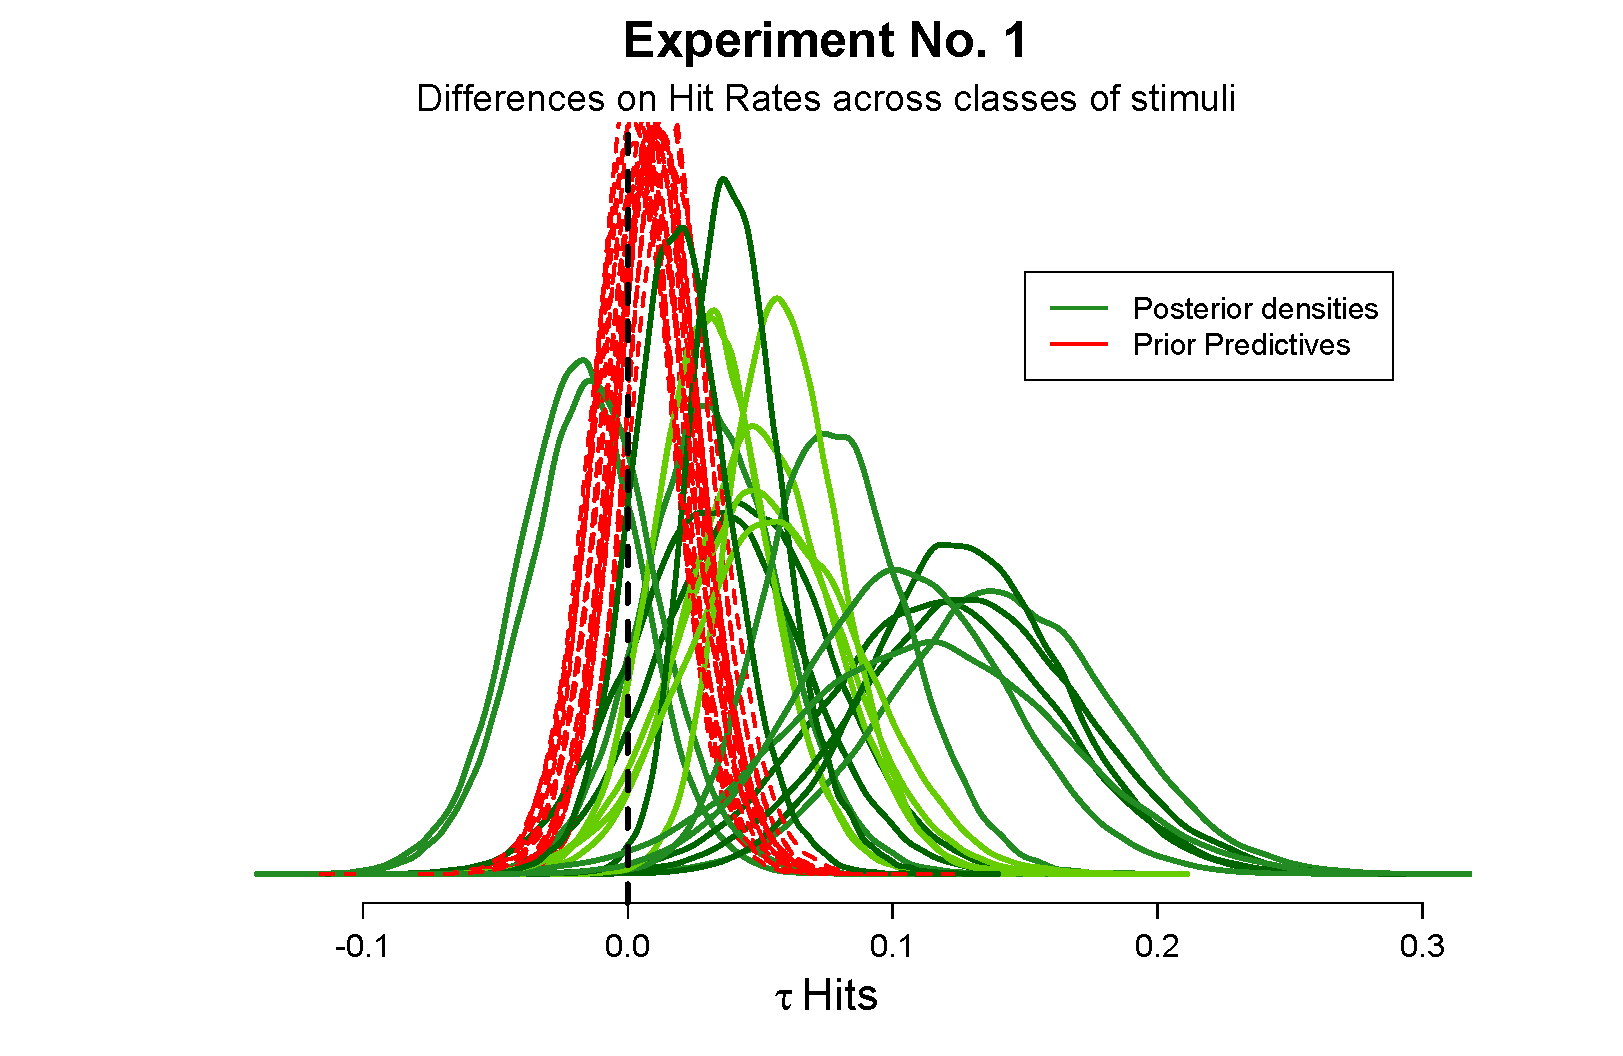
\includegraphics[width=0.45\linewidth]{Figures/3-Exp1_TauH.pdf}  & \hfill & 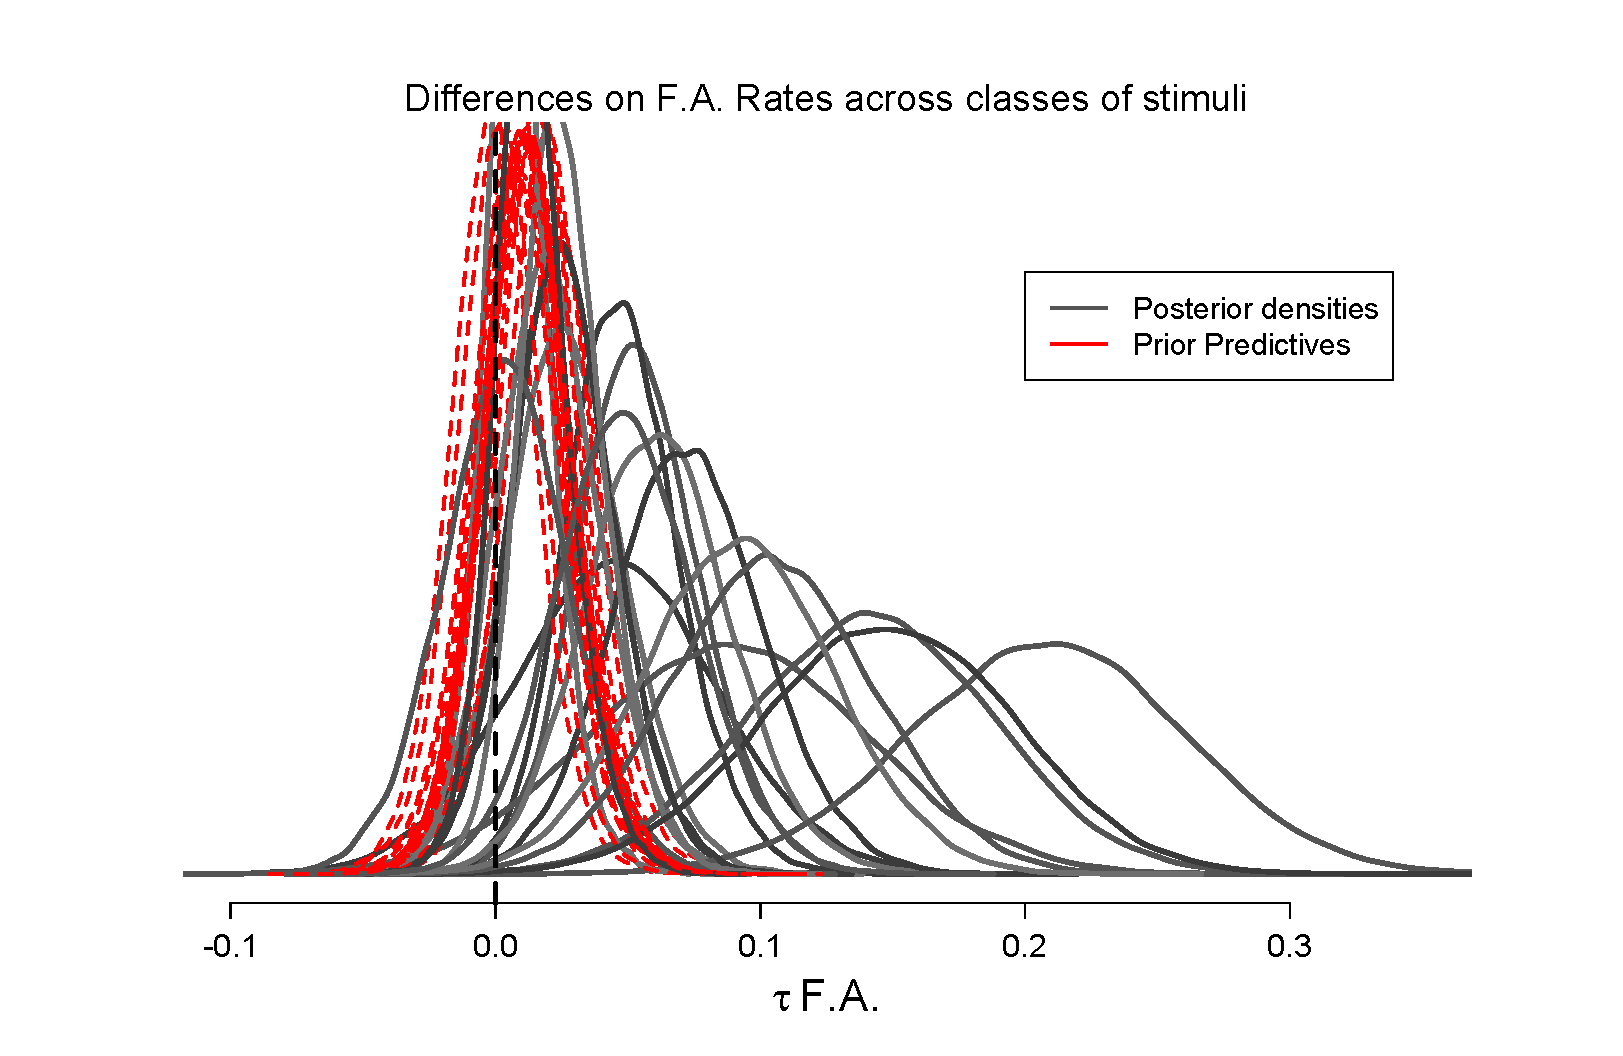
\includegraphics[width=0.45\linewidth]{Figures/3-Exp1_TauF.pdf}
\end{tabular}
\end{center}

\begin{center}
\begin{tabular}{ccc}
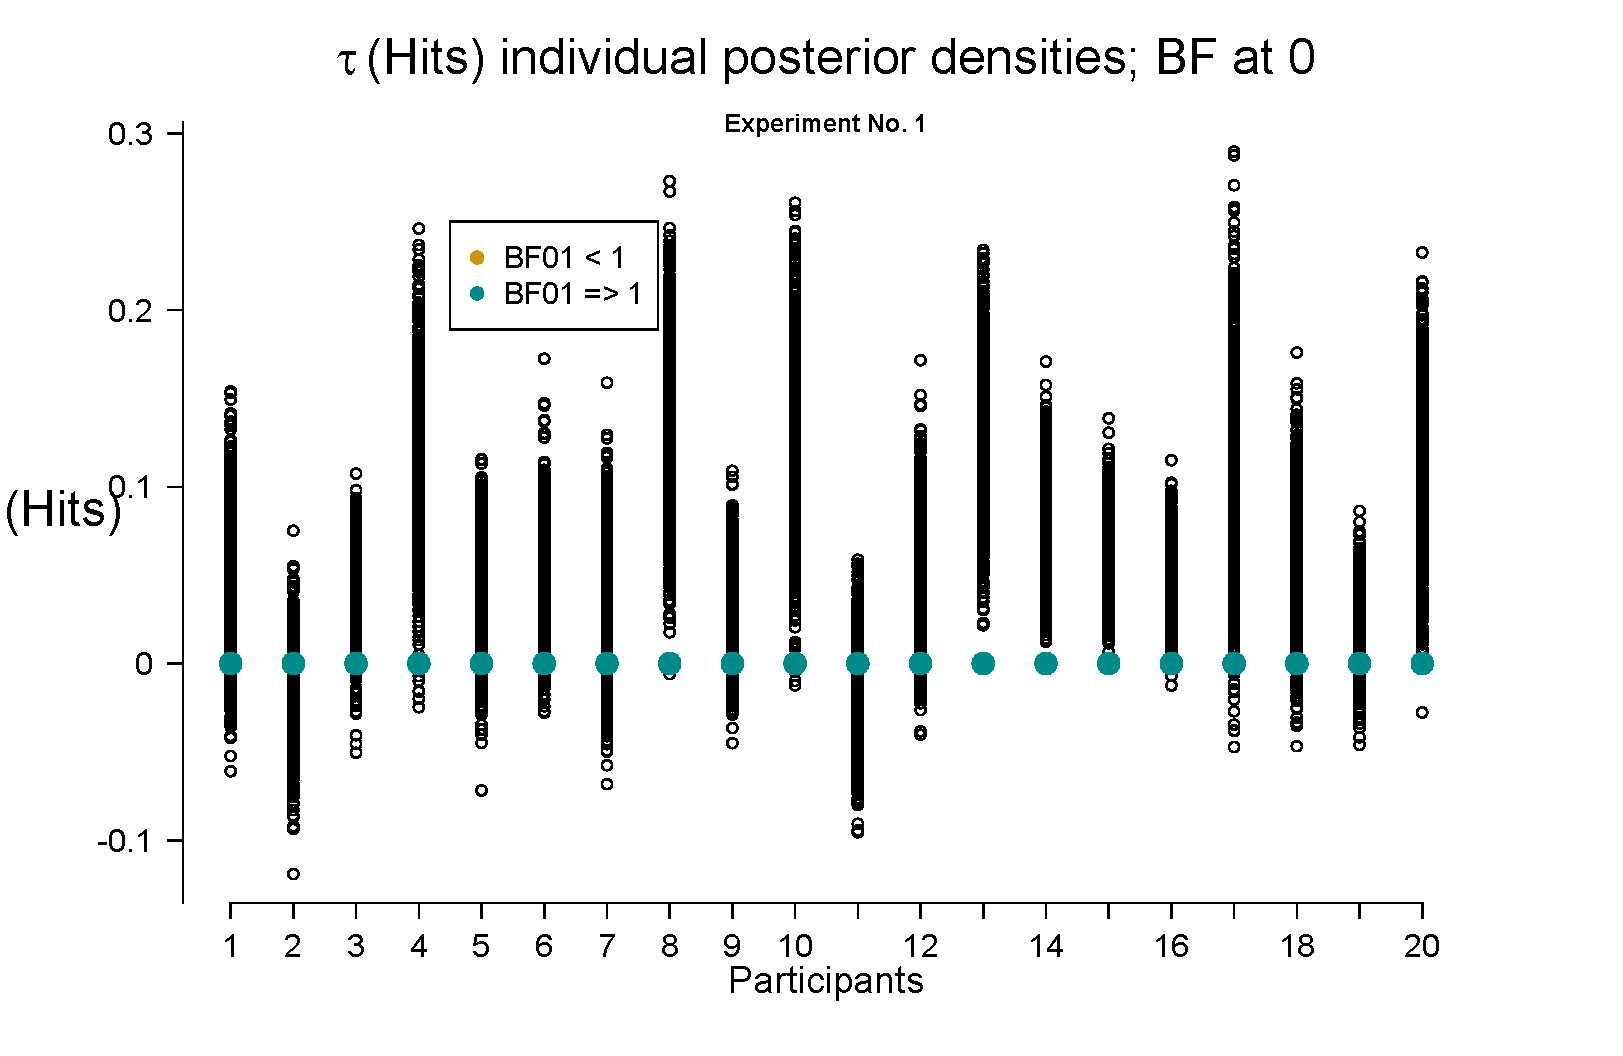
\includegraphics[width=0.45\linewidth]{Figures/3-Exp1_BFH0.pdf}  & \hfill & 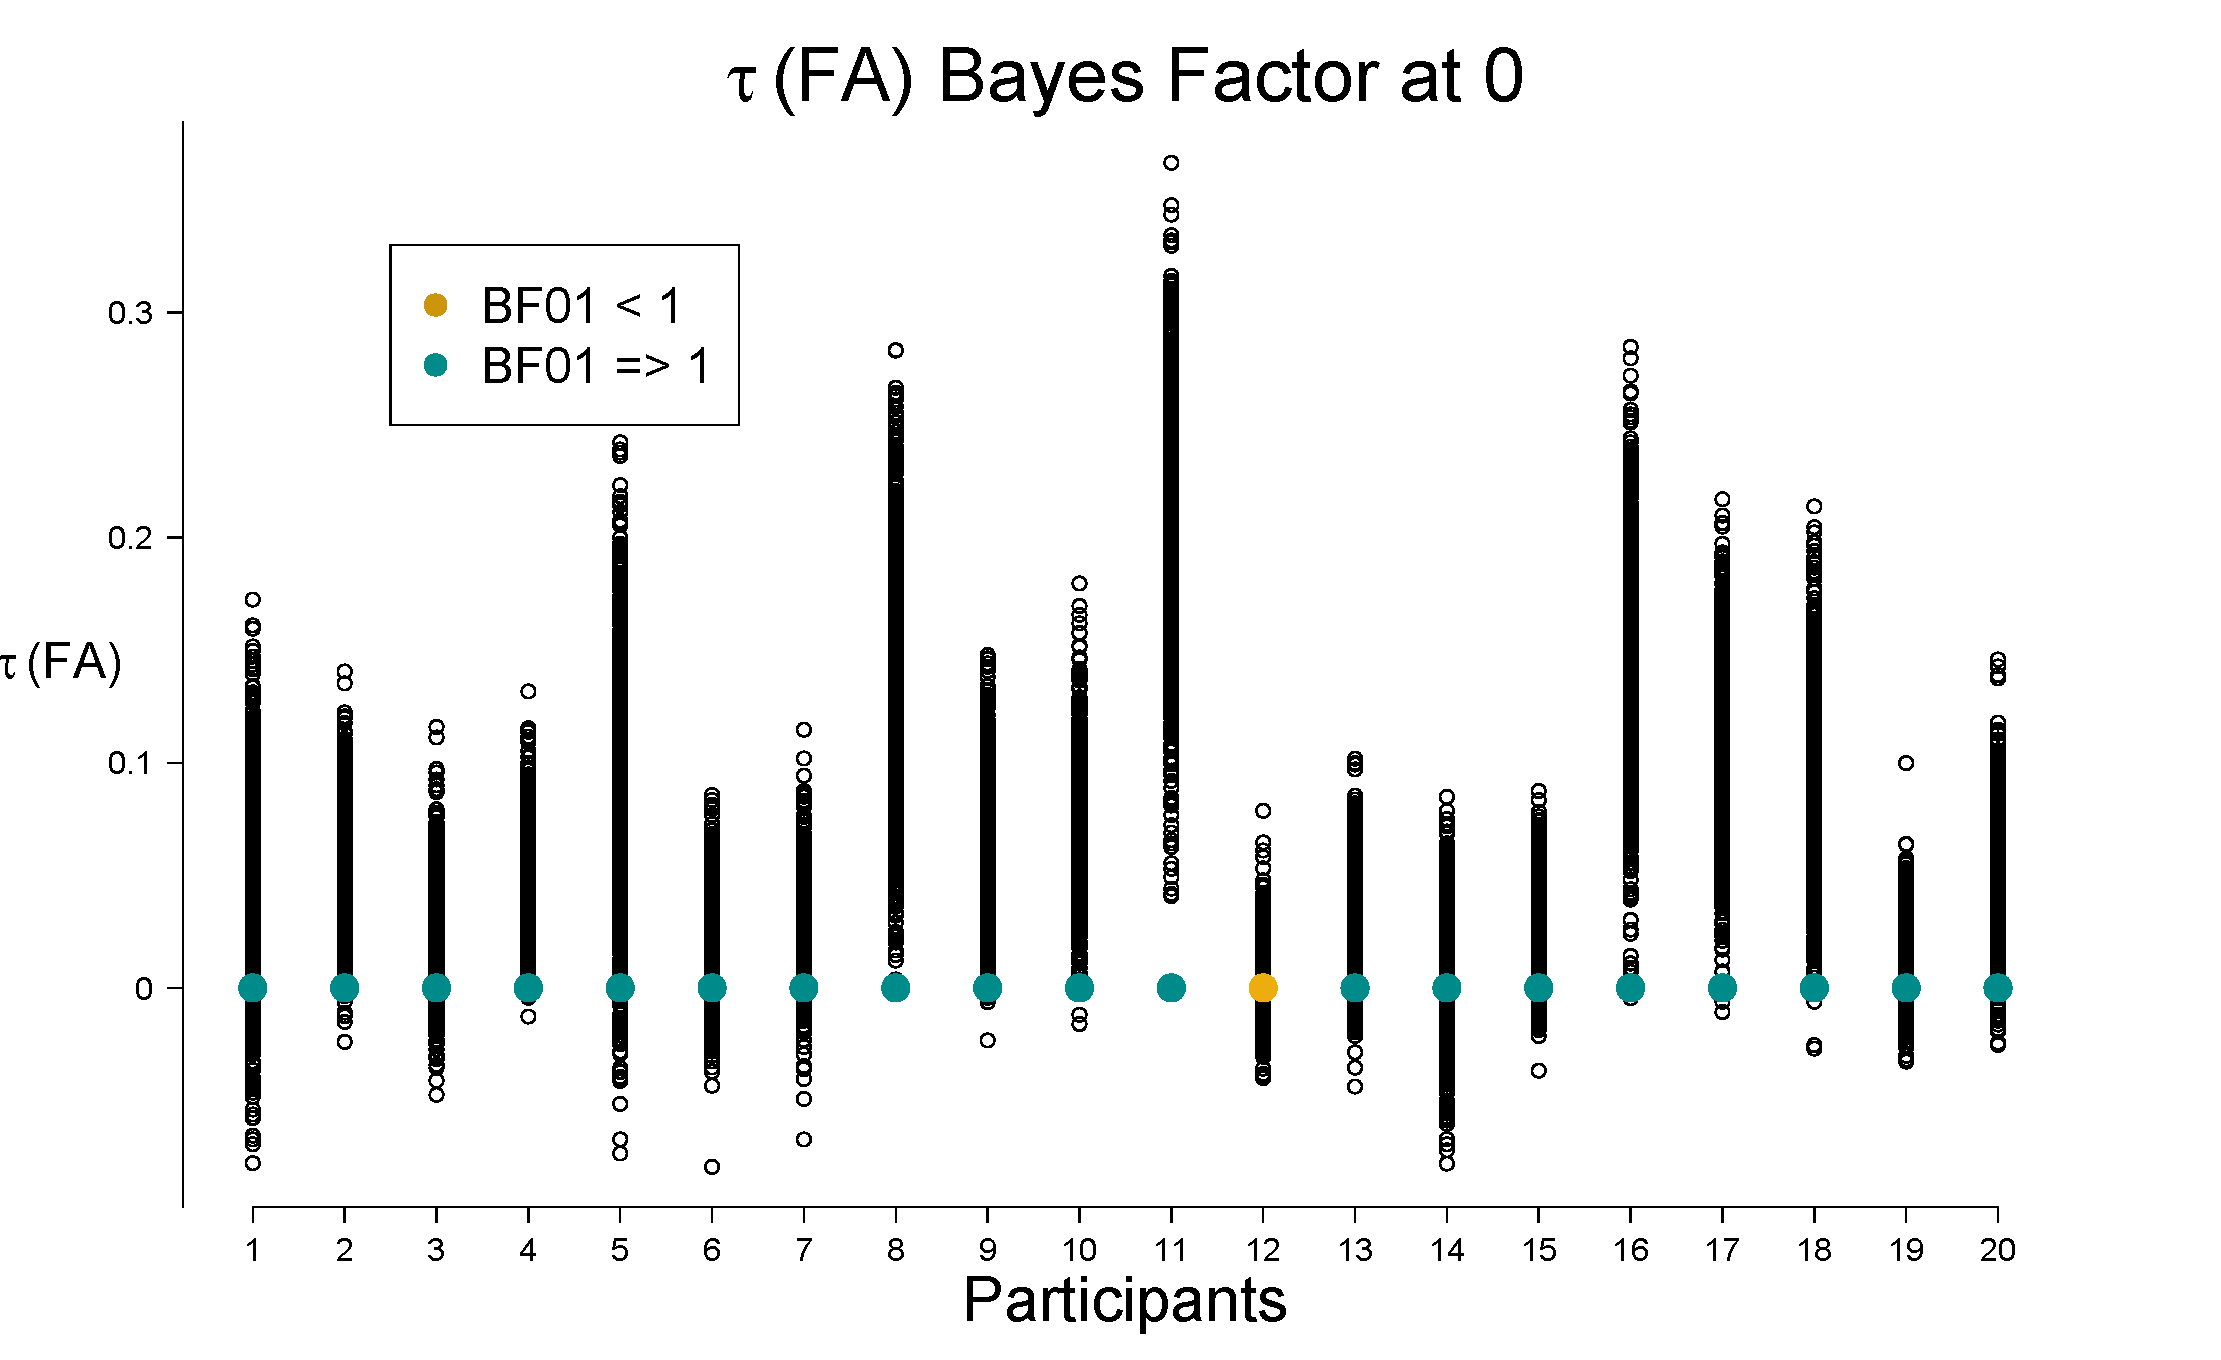
\includegraphics[width=0.45\linewidth]{Figures/3-Exp1_BFF0.pdf}
\end{tabular}
\end{center}

\begin{center}
\begin{tabular}{ccc}
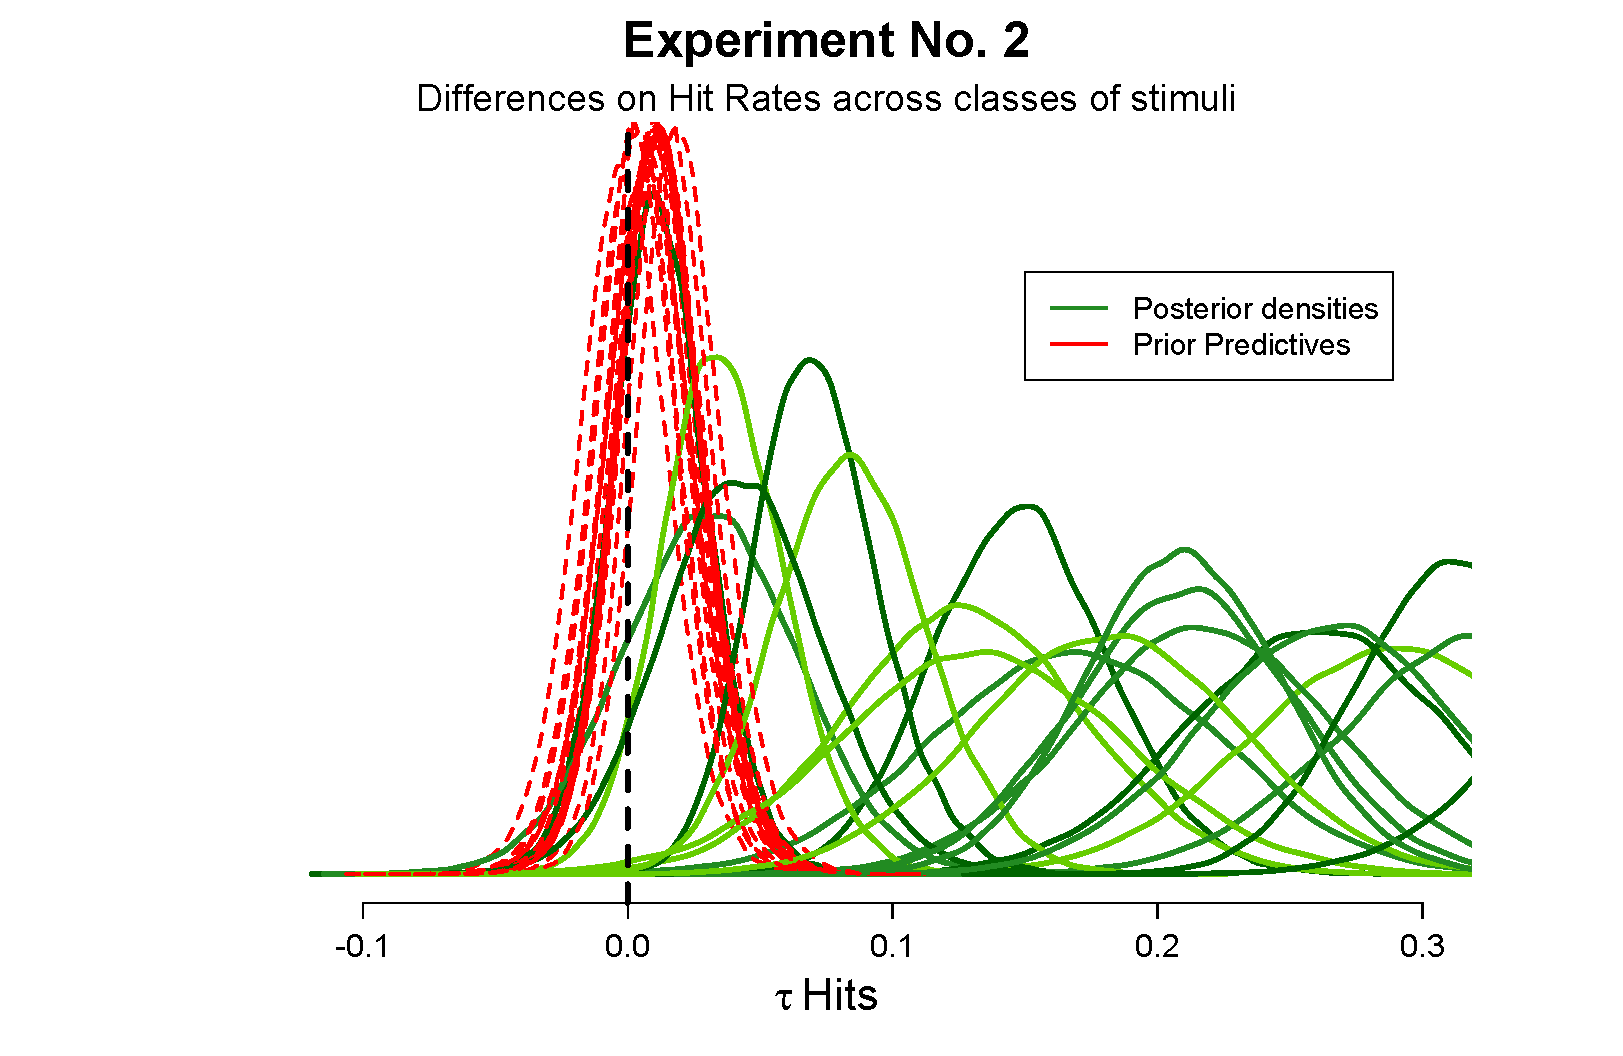
\includegraphics[width=0.45\linewidth]{Figures/3-Exp2_TauH.pdf}  & \hfill & 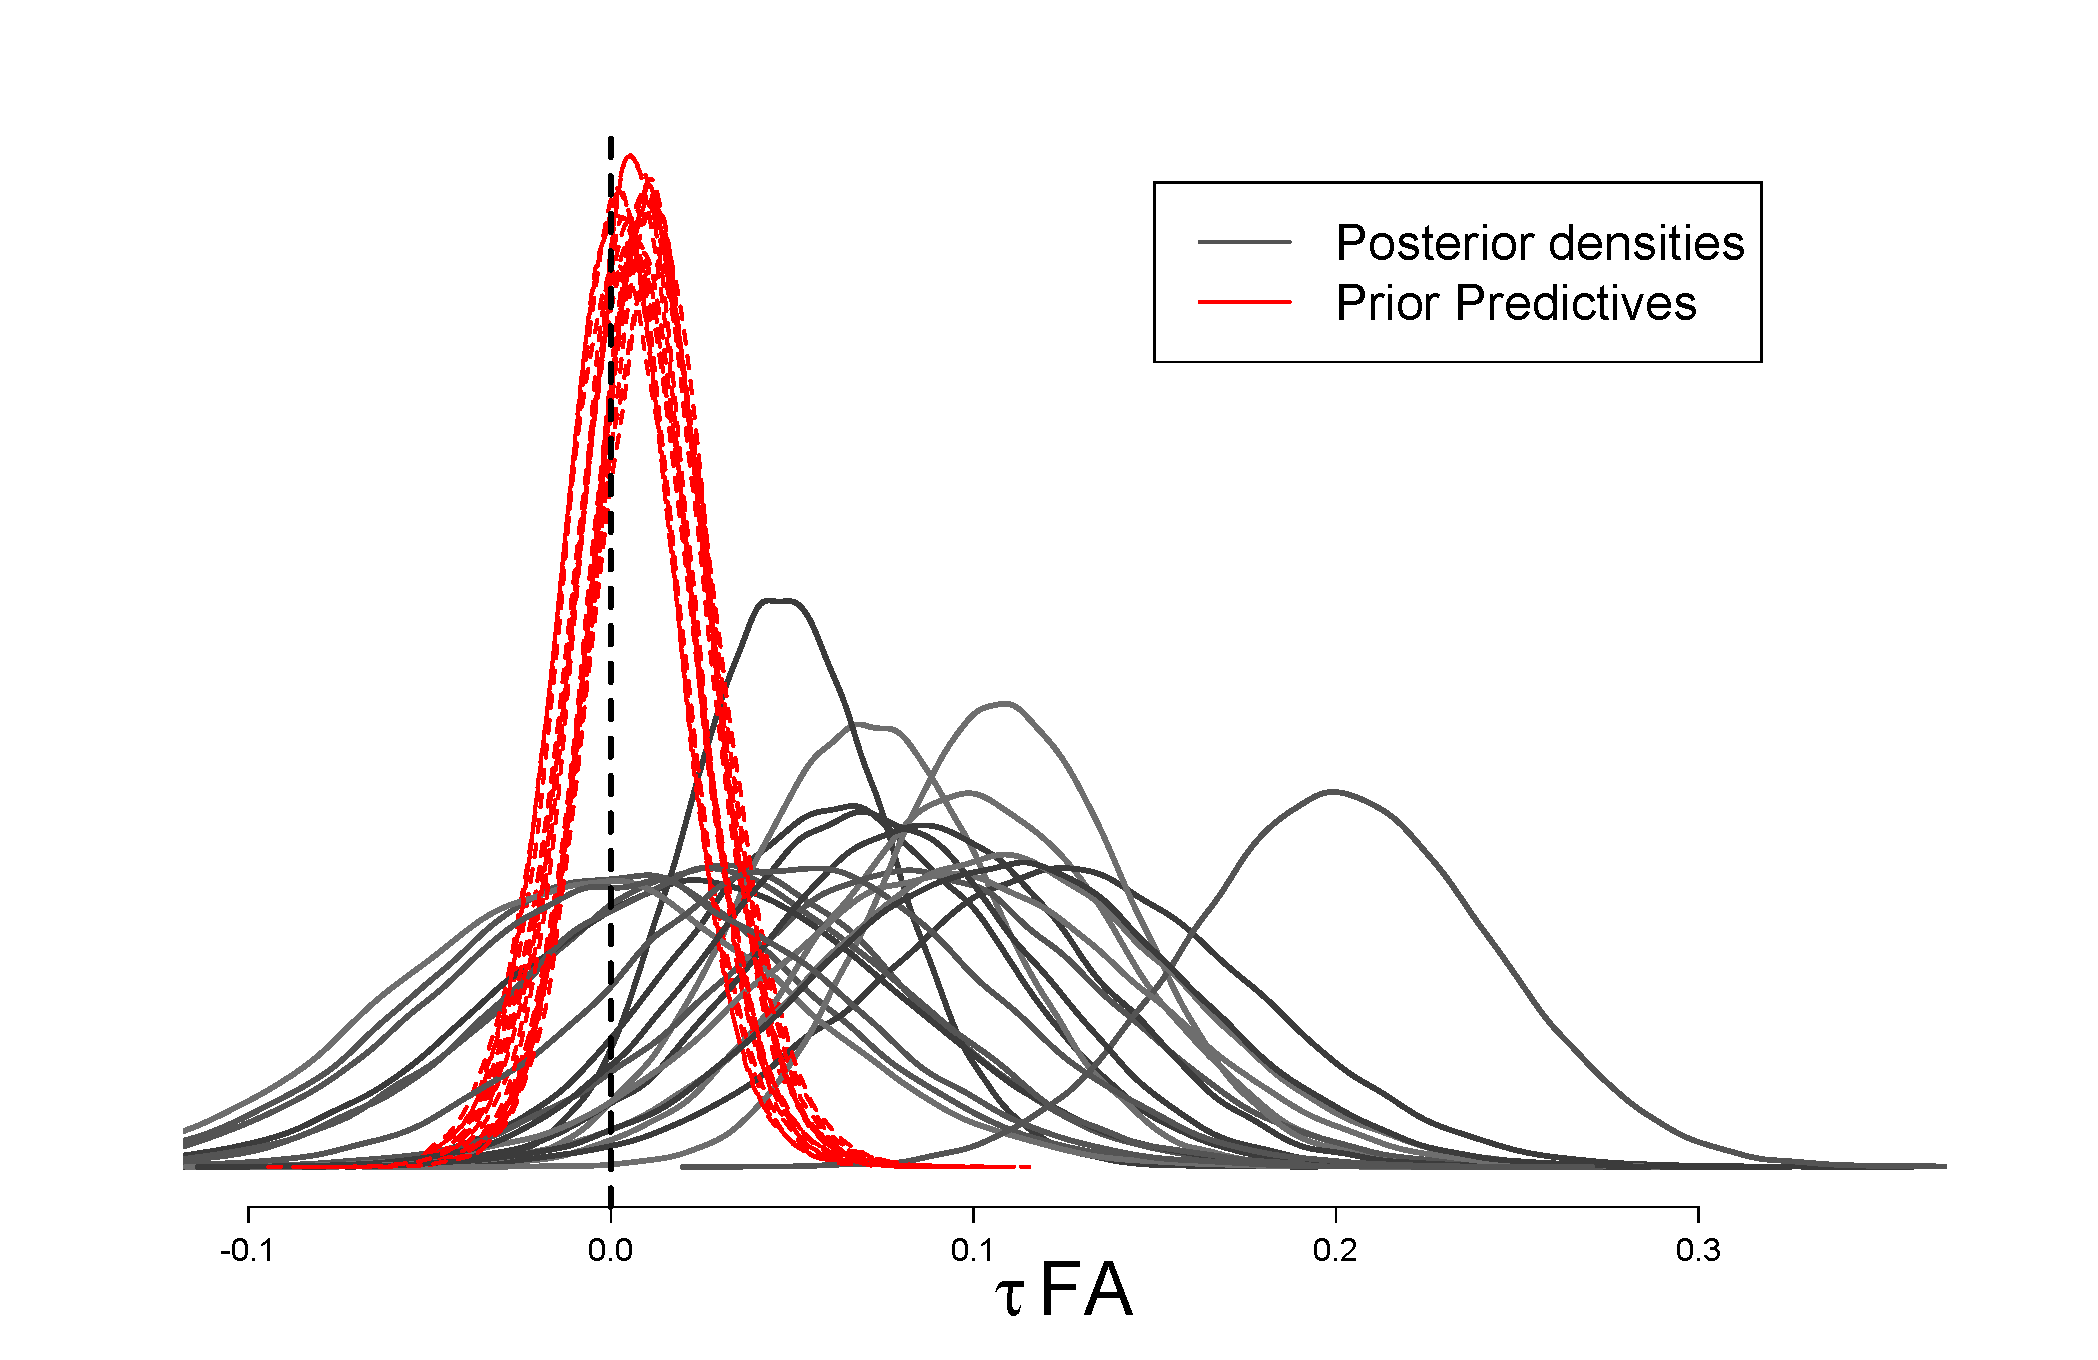
\includegraphics[width=0.45\linewidth]{Figures/3-Exp2_TauF.pdf}
\end{tabular}
\end{center}

\begin{center}
\begin{tabular}{ccc}
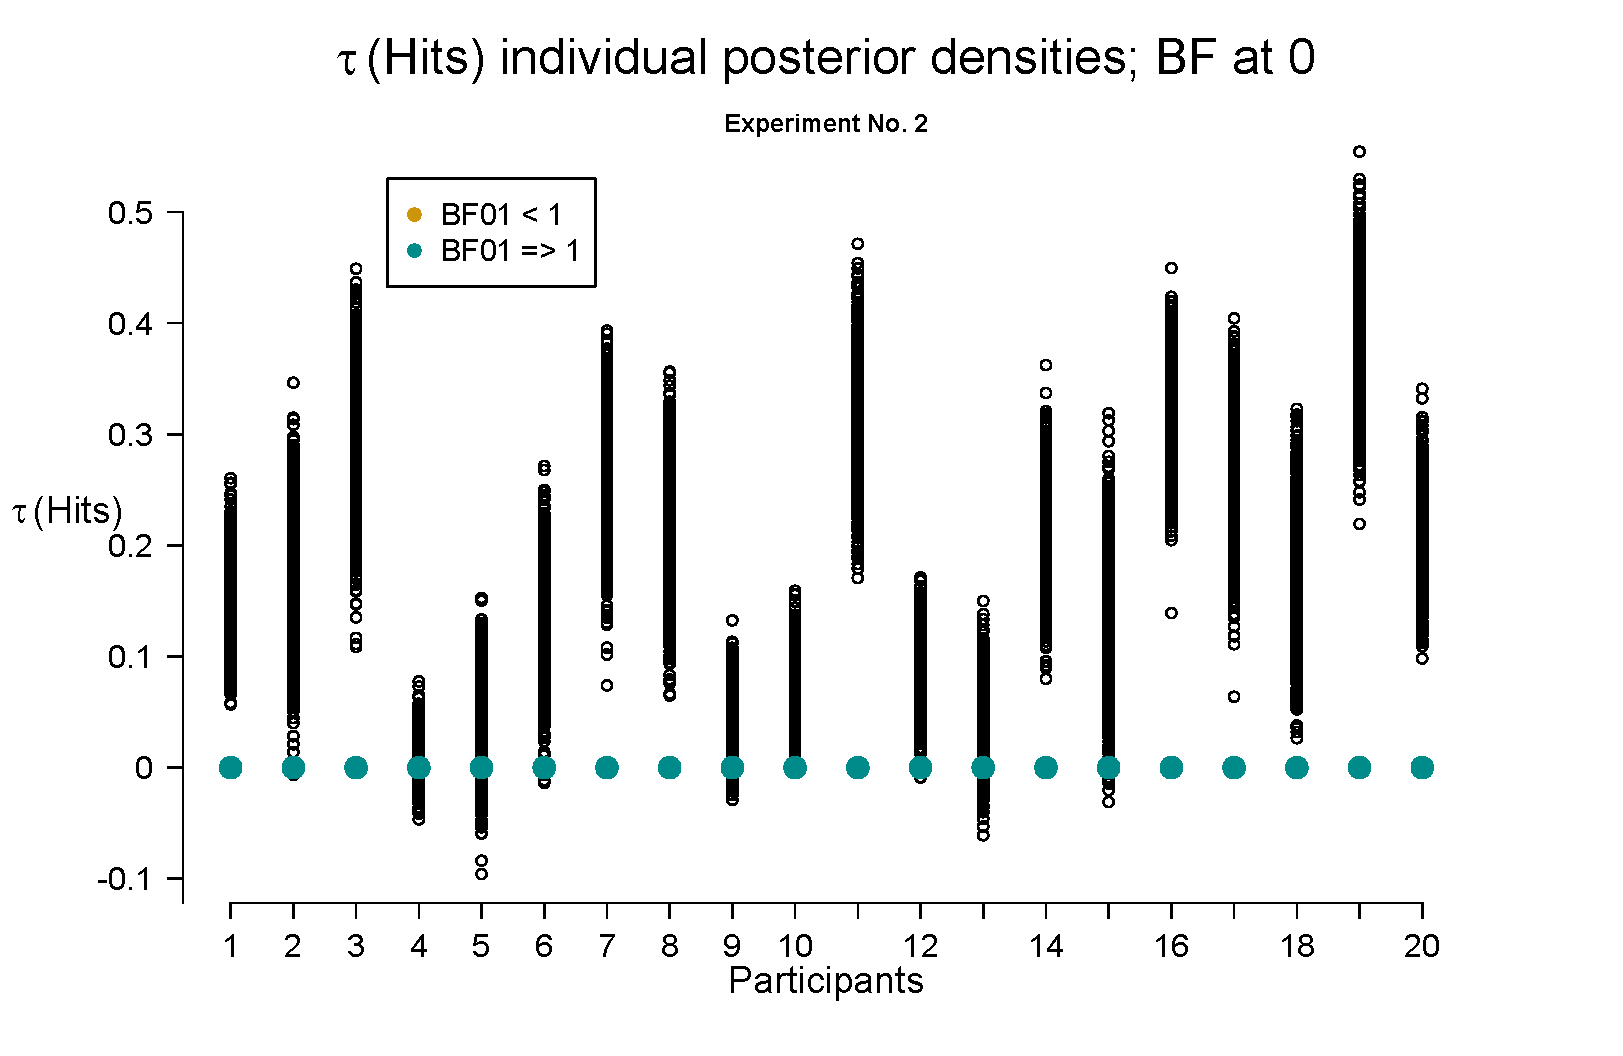
\includegraphics[width=0.45\linewidth]{Figures/3-Exp2_BFH0.pdf}  & \hfill & 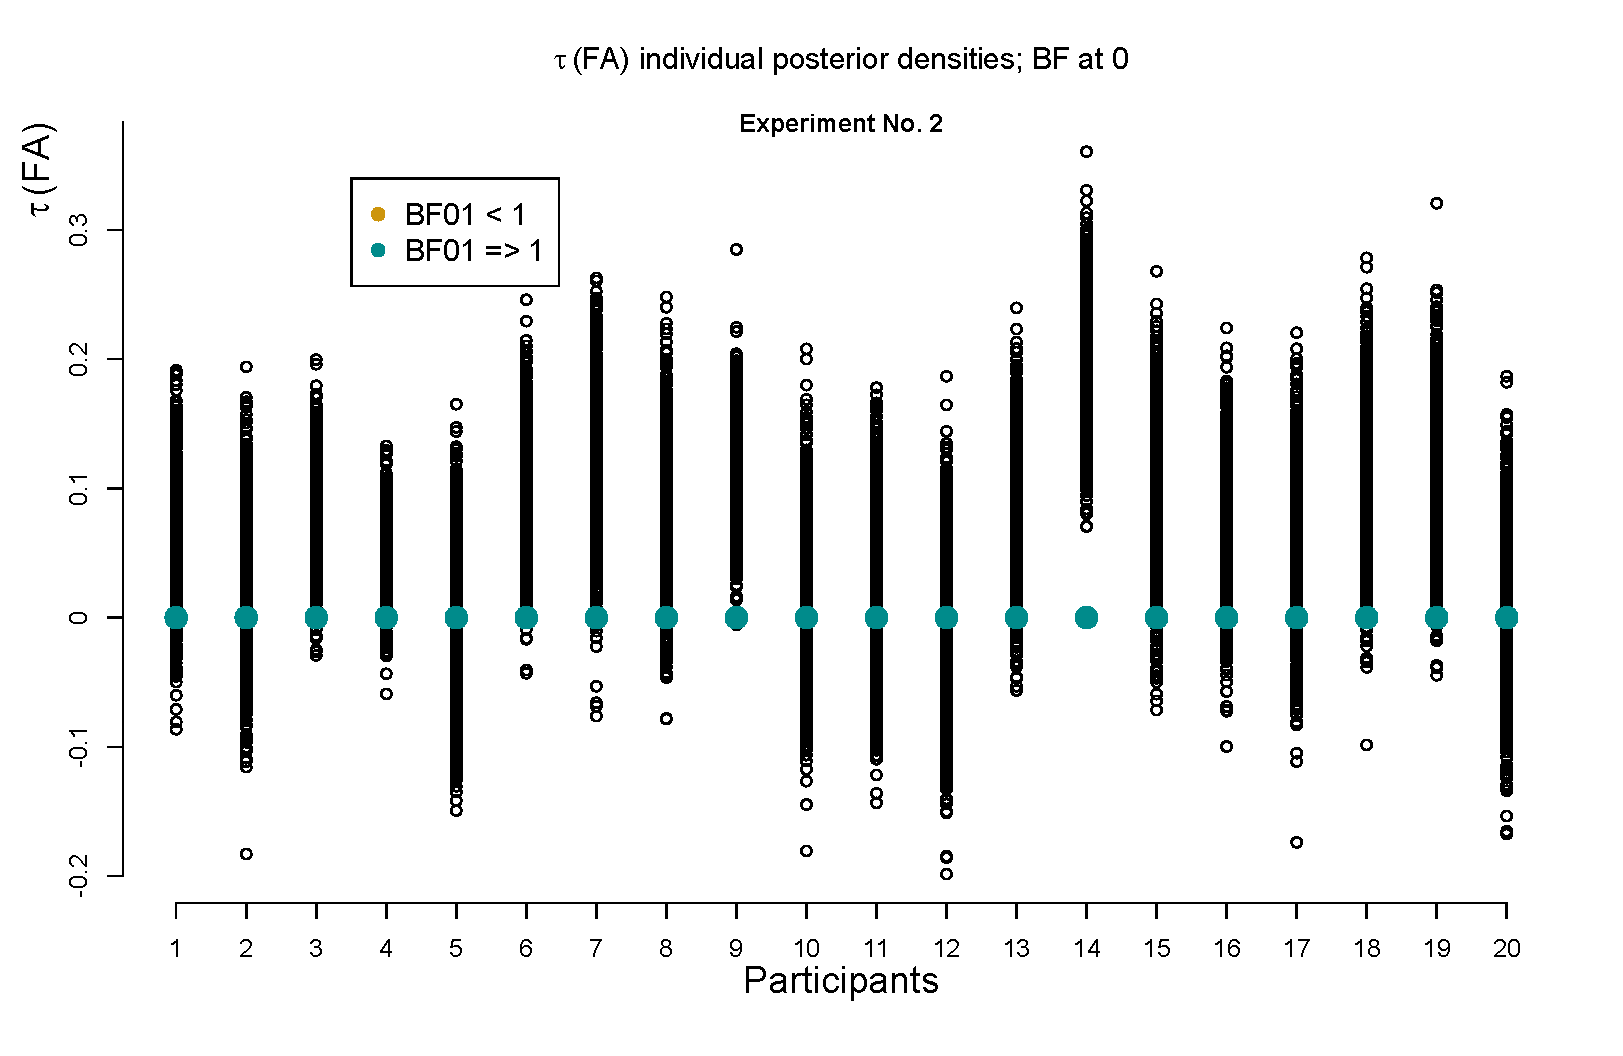
\includegraphics[width=0.45\linewidth]{Figures/3-Exp2_BFF0.pdf}
\end{tabular}
\end{center}


\end{alertblock}




%\begin{itemize}
%\item
%\end{itemize}


%----------------------------------------------------------------------------------------

\end{column} % End of column 2.2
\end{columns} % End of the split of column 2 - any content after this will now take up 2 columns width


\begin{column}{\threecolwid} % Begin a column which is two columns wide (column 2)

\setbeamercolor{block title}{fg=red,bg=white} % Change the block title color
\setbeamercolor{item}{fg=white}
\setbeamercolor{item projected}{fg=white,bg=white}
\setbeamercolor{block title}{fg=jblue,bg=white}
\setbeamercolor{block body}{fg=black,bg=white}
\begin{block}{Acknowledgments \& Contact Information}

\small{\rmfamily{This project was supported by PAPIIT-UNAM (). Thanks to Alexander Etz, J. M. Niño, Manuel Villarreal and José Luis Baroja for their inputs and help. \textbf{Website:} \href{www.bouzaslab25.com}{www.bouzaslab25.com}. \textbf{Email:} \href{mailto:adrifelcha@gmail.com}{adrifelcha@gmail.com}}} \\
\end{block}

\end{column}





%----------------------------------------------------------------------------------------

\begin{columns}[t,totalwidth=\twocolwid] % Split up the two columns wide column again

\begin{column}{\onecolwid} % The first column within column 2 (column 2.1)

%----------------------------------------------------------------------------------------

\end{column} % End of column 2.1

\end{columns} % End of the split of column 2

\end{column} % End of the second column

\begin{column}{\sepwid}\end{column} % Empty spacer column

\setlength{\onecolwid}{0.252\paperwidth} % Width of one column
\begin{column}{\onecolwid} % The third column

%----------------------------------------------------------------------------------------
%   CONCLUSION
%----------------------------------------------------------------------------------------

\setbeamercolor{block alerted title}{fg=white,bg=MidnightBlue} % Titulo
\setbeamercolor{block alerted body}{fg=black,bg=white} % Cuerpo
\begin{alertblock}{Contaminant Model}


\begin{center}
\begin{tabular}{ccc}
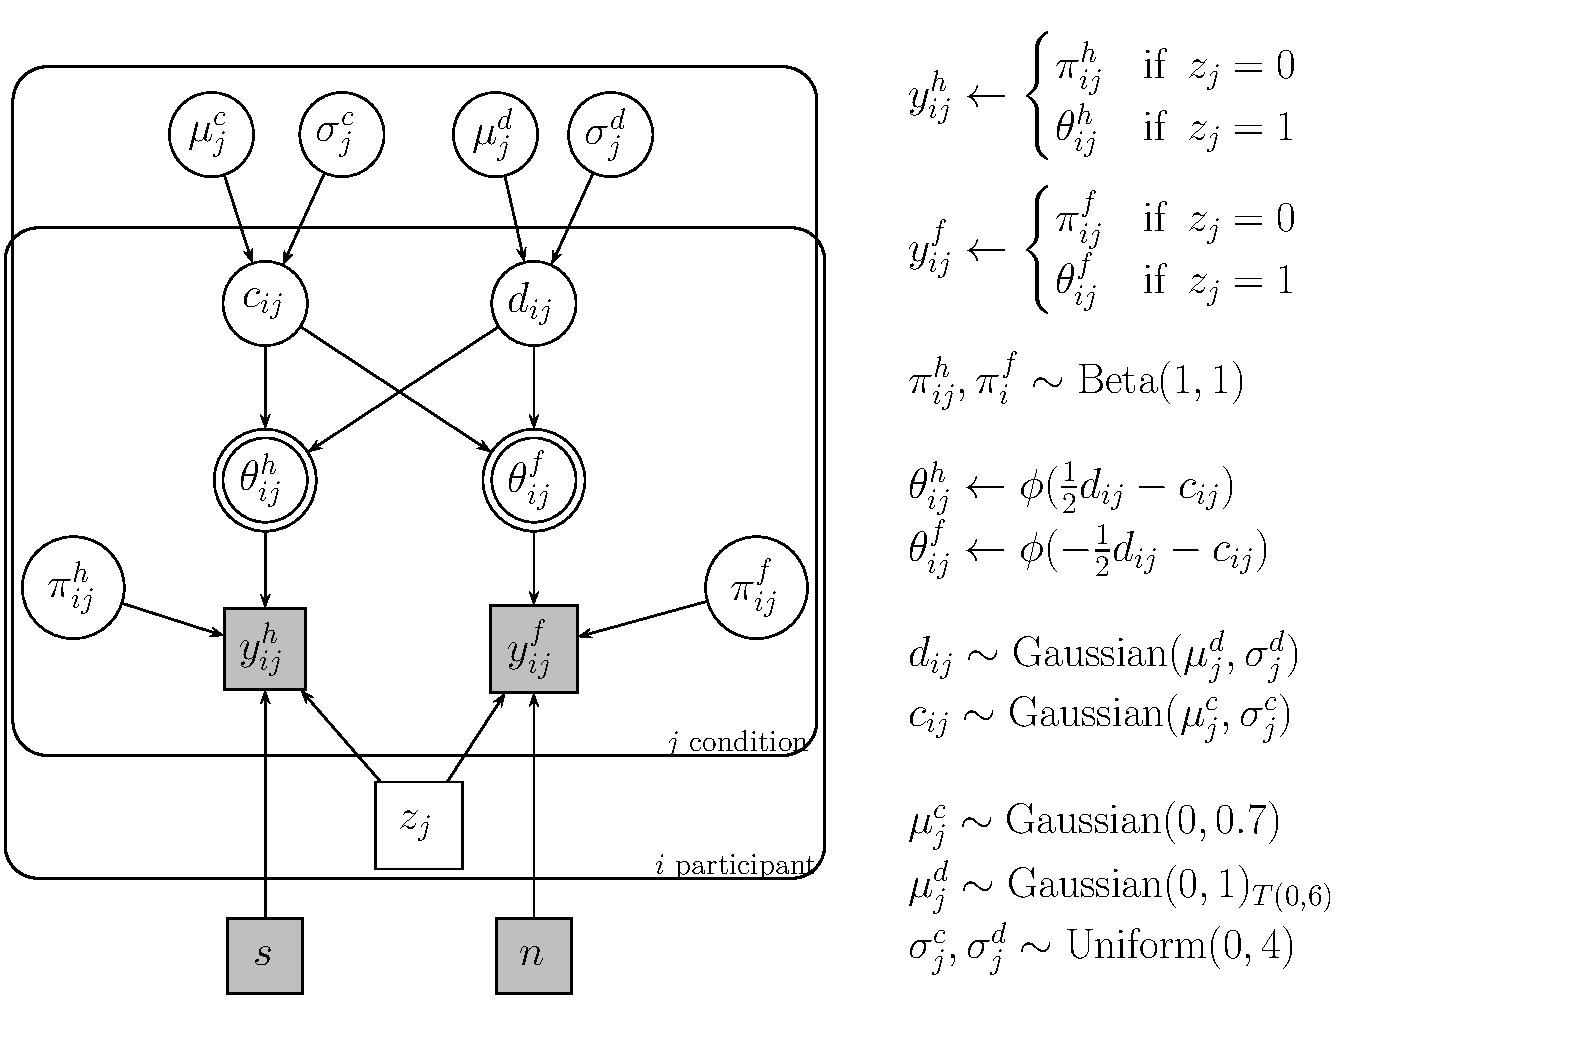
\includegraphics[width=0.75\linewidth]{Figures/4_Contaminant.pdf}
\end{tabular}
\end{center}

\end{alertblock}



\setbeamercolor{block alerted title}{fg=white,bg=Plum}
\setbeamercolor{block alerted body}{fg=black,bg=Plum!10}
%\setbeamercolor{block alerted title}{fg=white,bg=CadetBlue} % Change the alert block title colors
%\setbeamercolor{block alerted body}{fg=black,bg=white} % Change the alert block body colors
\begin{alertblock}{Discussion}

The present study is the first to show evidence of the Mirror Effect patterns of response on a SD task that does not involve recognition memory.\\

The perceptual task here presented lacked a pre-experimental phase where participants had the chance to manipulate how powerful were the illusions elicited in each condition. This suggests that there might be a much more basic principle regulating the Mirror Effect pattern of responses.

\end{alertblock}

%----------------------------------------------------------------------------------------
%   REFERENCES
%----------------------------------------------------------------------------------------

\setbeamercolor{item}{fg=white}
\setbeamercolor{item projected}{fg=white,bg=white}
\setbeamercolor{block alerted title}{fg=white,bg=Plum}
\setbeamercolor{block alerted body}{fg=black,bg=Plum!10}
\begin{alertblock}{References}

\setbeamercolor{item}{fg=WildStrawberry}
\setbeamercolor{item projected}{fg=white,bg=WildStrawberry}
\begin{itemize}
\item Glanzer, M., Adams, J. (1990) The Mirror Effect in Recognition Memory \: Data and Theory.\textit{Journal of Experimental Psychology: Learning, Memory and Cognition, 16} (1), 5-16.
\item Glanzer, M., Adams, J., Iverson, G. \& Kim, K. (1993) The Regularities of Recognition Memory. \textit{Psychological Review, 100} (3), 546-567.
\item Massaro, D., Anderson, N. (1971). Judgmental model of the Ebbinghaus Illusion. \textit{Journal of Experimental Psychology, 89}, 147 - 151.
\end{itemize}

%\nocite{*} % Insert publications even if they are not cited in the poster
%\small{\bibliographystyle{unsrt}
%\bibliography{sample}\vspace{0.75in}}

\end{alertblock}



\end{column} % End of the third column
\end{columns} % End of all the columns in the poster
\end{frame} % End of the enclosing frame
\end{document}

              